\documentclass{article}
\input{../../../LaTex/preamble/preamble_article.tex}


\title{高中物理}
\author{马祥芸}


\begin{document}
\maketitle
\tableofcontents
\zihao{-4}
\newpage

\section{科学常识}
\begin{enumerate}
    \item 亚里士多德认为物体下落的快慢与它的轻重(质量)有关,这种观念是错误的

          \vspace{-1em}

          \hspace{-1em}\begin{adjustbox}{minipage=0.86\linewidth, bgcolor=gray!20, padding=1em}
              \small % 将字号变小为 small
              亚里士多德(公元前$384\sim322$年)提出过许多错误的观点和理论,但是我们应该辩证地看待,保持尊重
          \end{adjustbox}

          \vspace{-1em}

    \item 伽利略通过\textbf{比萨斜塔实验},论证了自由落体的物体下落快慢与轻重(质量)无关
    \item 伽利略的\textbf{斜面滑块实验}论证了小球的匀加速运动的大小与斜面倾斜程度无关
    \item 牛顿三定律:
          \begin{itemize}
              \item \textbf{第一定律(惯性定律):} $ F = 0 \quad \lra \quad $物体保持静止或匀速运动
              \item \textbf{第二定律(运动定律):} $ \va{F} = m \, \va{a} $
              \item \textbf{第三定律(作用与反作用定律):} $ \va{F}_{AB} = - \va{F}_{BA} $ 力是成对存在的,大小相等方向相反
          \end{itemize}
    \item 平行四边形定则: 保持匀速或静止的物体,力的合成为\textbf{零向量$\va{0}$}
    \item 托勒密地心说: 地球是宇宙的中心,是静止的,太阳和月亮以及其他星体围绕地球转
    \item 哥白尼日心说: 太阳是宇宙的中心,地球和其他行星围绕太阳转
    \item 第谷: 精确的天文数据为日后开普勒的行星运动定律的发现提供了重要的\textbf{观测依据}
    \item 开普勒行星运动定律:
          \begin{itemize}
              \item \textbf{第一定律(椭圆轨道定律):} 运动的轨道是椭圆,太阳位于椭圆的一个焦点上
              \item \textbf{第二定律(面积定律):} 行星在相等时间内,在轨道上扫过的面积相等
              \item \textbf{第三定律(调和定律):} $ \frac{a^{3}}{T^{2}} = k $ 其中$a$是轨道半长轴
          \end{itemize}
    \item 胡克等科学家: 行星绕太阳运动是因为受到了\textbf{引力},甚至证明了与距离的二次方成反比
    \item 牛顿万有引力定律: $ \va{F} = G\dfrac{m_{1}m_{2}}{\va{r}^{2}}$
    \item 卡文迪什通过\textbf{扭秤实验}测量了万有引力常量$G = 6.67 \cross 10^{-11} \, N \vdot m^{2}/kg^{2} $

          \vspace{-1em}

          \hspace{-1em}\begin{adjustbox}{minipage=0.865\linewidth, bgcolor=gray!20, padding=1em}
              \small % 将字号变小为 small
              石英丝连接细杆,两端放置等大质量球,在两球附近放置两大质量球产生引力矩,用光线反射法放大扭转

              \vspace{-1em}

              $$ \theta \propto \text{力矩} \quad \lra  \quad k\theta = 2F_{G}L \quad (k\text{为比例系数需提前测量}) $$
          \end{adjustbox}

          \vspace{-1em}

    \item 亚当斯和勒维耶利用万有引力定律计算出了"新"行星的轨道
    \item 伽勒和勒维耶发现了这颗行星,后被命名为海王星
    \item 哈雷利用万有引力预言了同一彗星的按时回归,后被命名为"哈雷彗星"
    \item 钱学森被誉为"中国航天之父",地球同步卫星的(赤道)轨道高度$36000 \,km$
    \item 阿姆斯特朗:人类登月第一人 \quad 杨利伟:中国登月第一人
\end{enumerate}

\vspace{2em}

\section{匀变速直线运动问题}

\subsection{中间时刻/平均速度}
中间时刻速度$v_{\frac{t}{2}}$与平均速度$\overline{v}$是同一个值
$$
    v_{\frac{t}{2}} = v_{0} + \frac{at}{2} = \frac{v_{0}}{2} +  (\frac{v_{0}}{2} + \frac{at}{2})   = \frac{v_{0}+v_{t}}{2} = \overline{v}
$$

中间位置速度

\begin{numcases}{}
    \label{1} 2 a\frac{x}{2} = v_{\frac{x}{2}}^{2} - v_{0}^{2}  \\
    \label{2} 2 a\frac{x}{2} = v_{t}^{2} - v_{\frac{x}{2}}^{2}
\end{numcases}

由方程$(1) - (2)$ 得到 $ v_{\frac{x}{2}} = \sqrt{\frac{v_{0}^{2} + v_{t}^{2}}{2}} $

\subsection{纸带加速度问题}
纸带的特点,每个计时点的时间间隔相同均为$T$,且$x_{n}$规定的是第$n$个时间间隔内的位移,并非到起点的距离

\begin{corollary*}
    相邻位移之间的差为$aT^{2}$,等时位移比例式为$x_{1}:x_{2}:x_{3} : \dots : x_{n} = 1:3:5: \dots :2n-1  $
\end{corollary*}
\begin{proof}
    \begin{align*}
        x_{n} = \frac{1}{2}a (nT)^{2} -  \frac{1}{2}a [(n-1)T]^{2} & = aT^{2} (\frac{2n-1}{2}) \\
        x_{n-1}                                                    & = aT^{2} (\frac{2n-3}{2}) \\
        x_{n} - x_{n-1}                                            & = aT^{2}
    \end{align*}
\end{proof}

\begin{corollary*}
    等位移比例式子($1m$,$2m$,$3m \dots$)    \\
    前$1m,2m,3m \dots n \, m$所用时间比为$1:\sqrt{2}:\sqrt{3}:\dots:\sqrt{n}$,若是第$i\,m$内则向前减一个就行
    \begin{proof}
        \begin{align*}
            1 & = \frac{1}{2}a t_{1}^{2} \lra t_{1} =\sqrt{\frac{2}{a}} \vdot \sqrt{1} \\
            2 & = \frac{1}{2}a t_{2}^{2} \lra t_{2} =\sqrt{\frac{2}{a}} \vdot \sqrt{2} \\
            3 & = \frac{1}{2}a t_{3}^{2} \lra t_{3} =\sqrt{\frac{2}{a}} \vdot \sqrt{3} \\
            n & = \frac{1}{2}a t_{n}^{2} \lra t_{n} =\sqrt{\frac{2}{a}} \vdot \sqrt{n} \\
        \end{align*}
    \end{proof}
\end{corollary*}

\vspace{2em}

\section{机械振动}
\subsection{简谐振动}
\begin{itemize}
    \item 定义: 具有平衡位置,回复力形如$F_{\text{回}} = -kx$(来自合外力或其分力)
    \item 振子方程: $\sin{(\omega t + \varphi)}$
    \item 同侧法: 质点振动速度方向$v_{f}$与波传播方向$u$在正弦函数线的同一侧
    \item 摆周期: $T = 2\pi \sqrt{\frac{L}{g}}$
    \item 受迫振动:在周期性外力的持续作用下而进行的振动称为\textbf{受迫振动}

          \hspace{4.7em}振动稳定后其\textbf{频率}等于外力驱动频率
    \item 等效绳长与等效加速度问题:
          \begin{itemize}
              \item 等效绳长: 确定为简谐振动,通过几何关系确定摆心
              \item 等效加速度: 主要区别电场摆和电梯摆,后者需要变换参考系(非惯性力)
          \end{itemize}
    \item  造成波的多解性的三大原因:
          \begin{itemize}
              \item \textbf{波的周期性:}\hspace{1em}
                    $\begin{cases}
                            \text{时间周期性:时间间隔}\triangle t \text{与周期} T \text{的关系不明确} \\
                            \text{空间周期性:波传播距离}\triangle x \text{与波长} \lambda \text{的关系不明确}
                        \end{cases}$

              \item \textbf{波的双向性:}\hspace{1em}
                    $\begin{cases}
                            \text{传播方向双向性:波的传播方向不确定} \\
                            \text{振动方向双向性:质点振动方向不确定}
                        \end{cases}$

              \item \textbf{波形隐含性:}\hspace{1em}
                    $\begin{cases}
                            \text{在波动问题中,有时只给出几个特殊点} \\
                            \text{(大多是两个特殊的点)的运动状态,其余信息均处于隐含状态}
                        \end{cases}$
          \end{itemize}
\end{itemize}

\vspace{2em}


\subsection{数学准备}
\begin{formal}
    \begin{itemize}
        \item 展开
              $$ \sin{(\theta \pm \beta)} = \sin{\theta}\cos{\theta} \pm \cos{\theta}\sin{\theta} $$
              $$ \cos{(\theta \pm \beta)} = \cos{\theta}\cos{\beta} \mp \sin{\theta}\sin{\beta} $$
              $$ \tan{(\theta \pm \beta)} = \dfrac{\tan{\theta} \pm \tan{\beta}}{1 \mp \tan{\theta}\tan{\beta}}$$

        \item 互余($\theta + \beta = \frac{\pi}{2}$)
              $$
                  \sin{\theta} = \cos{\beta}  \quad   \tan{\theta} = \frac{1}{\tan{\beta}}
              $$

        \item 互补($\theta + \beta = \pi$)
              $$
                  \sin{\theta} = \sin{\beta} \quad \cos{\theta} = - \cos{\beta}
                  \quad \tan{\theta} = - \tan{\beta}
              $$
        \item 半周期与奇偶性
              $$
                  \sin{(\theta \pm \pi)} = -\sin{\theta}   \quad   \sin{(\theta - \beta)} = - \sin{(\beta - \theta)}
              $$

              $$
                  \cos{(\theta \pm \pi)} = -\cos{\theta}   \quad   \cos{(\theta - \beta)} =  \cos{(\beta - \theta)}
              $$

              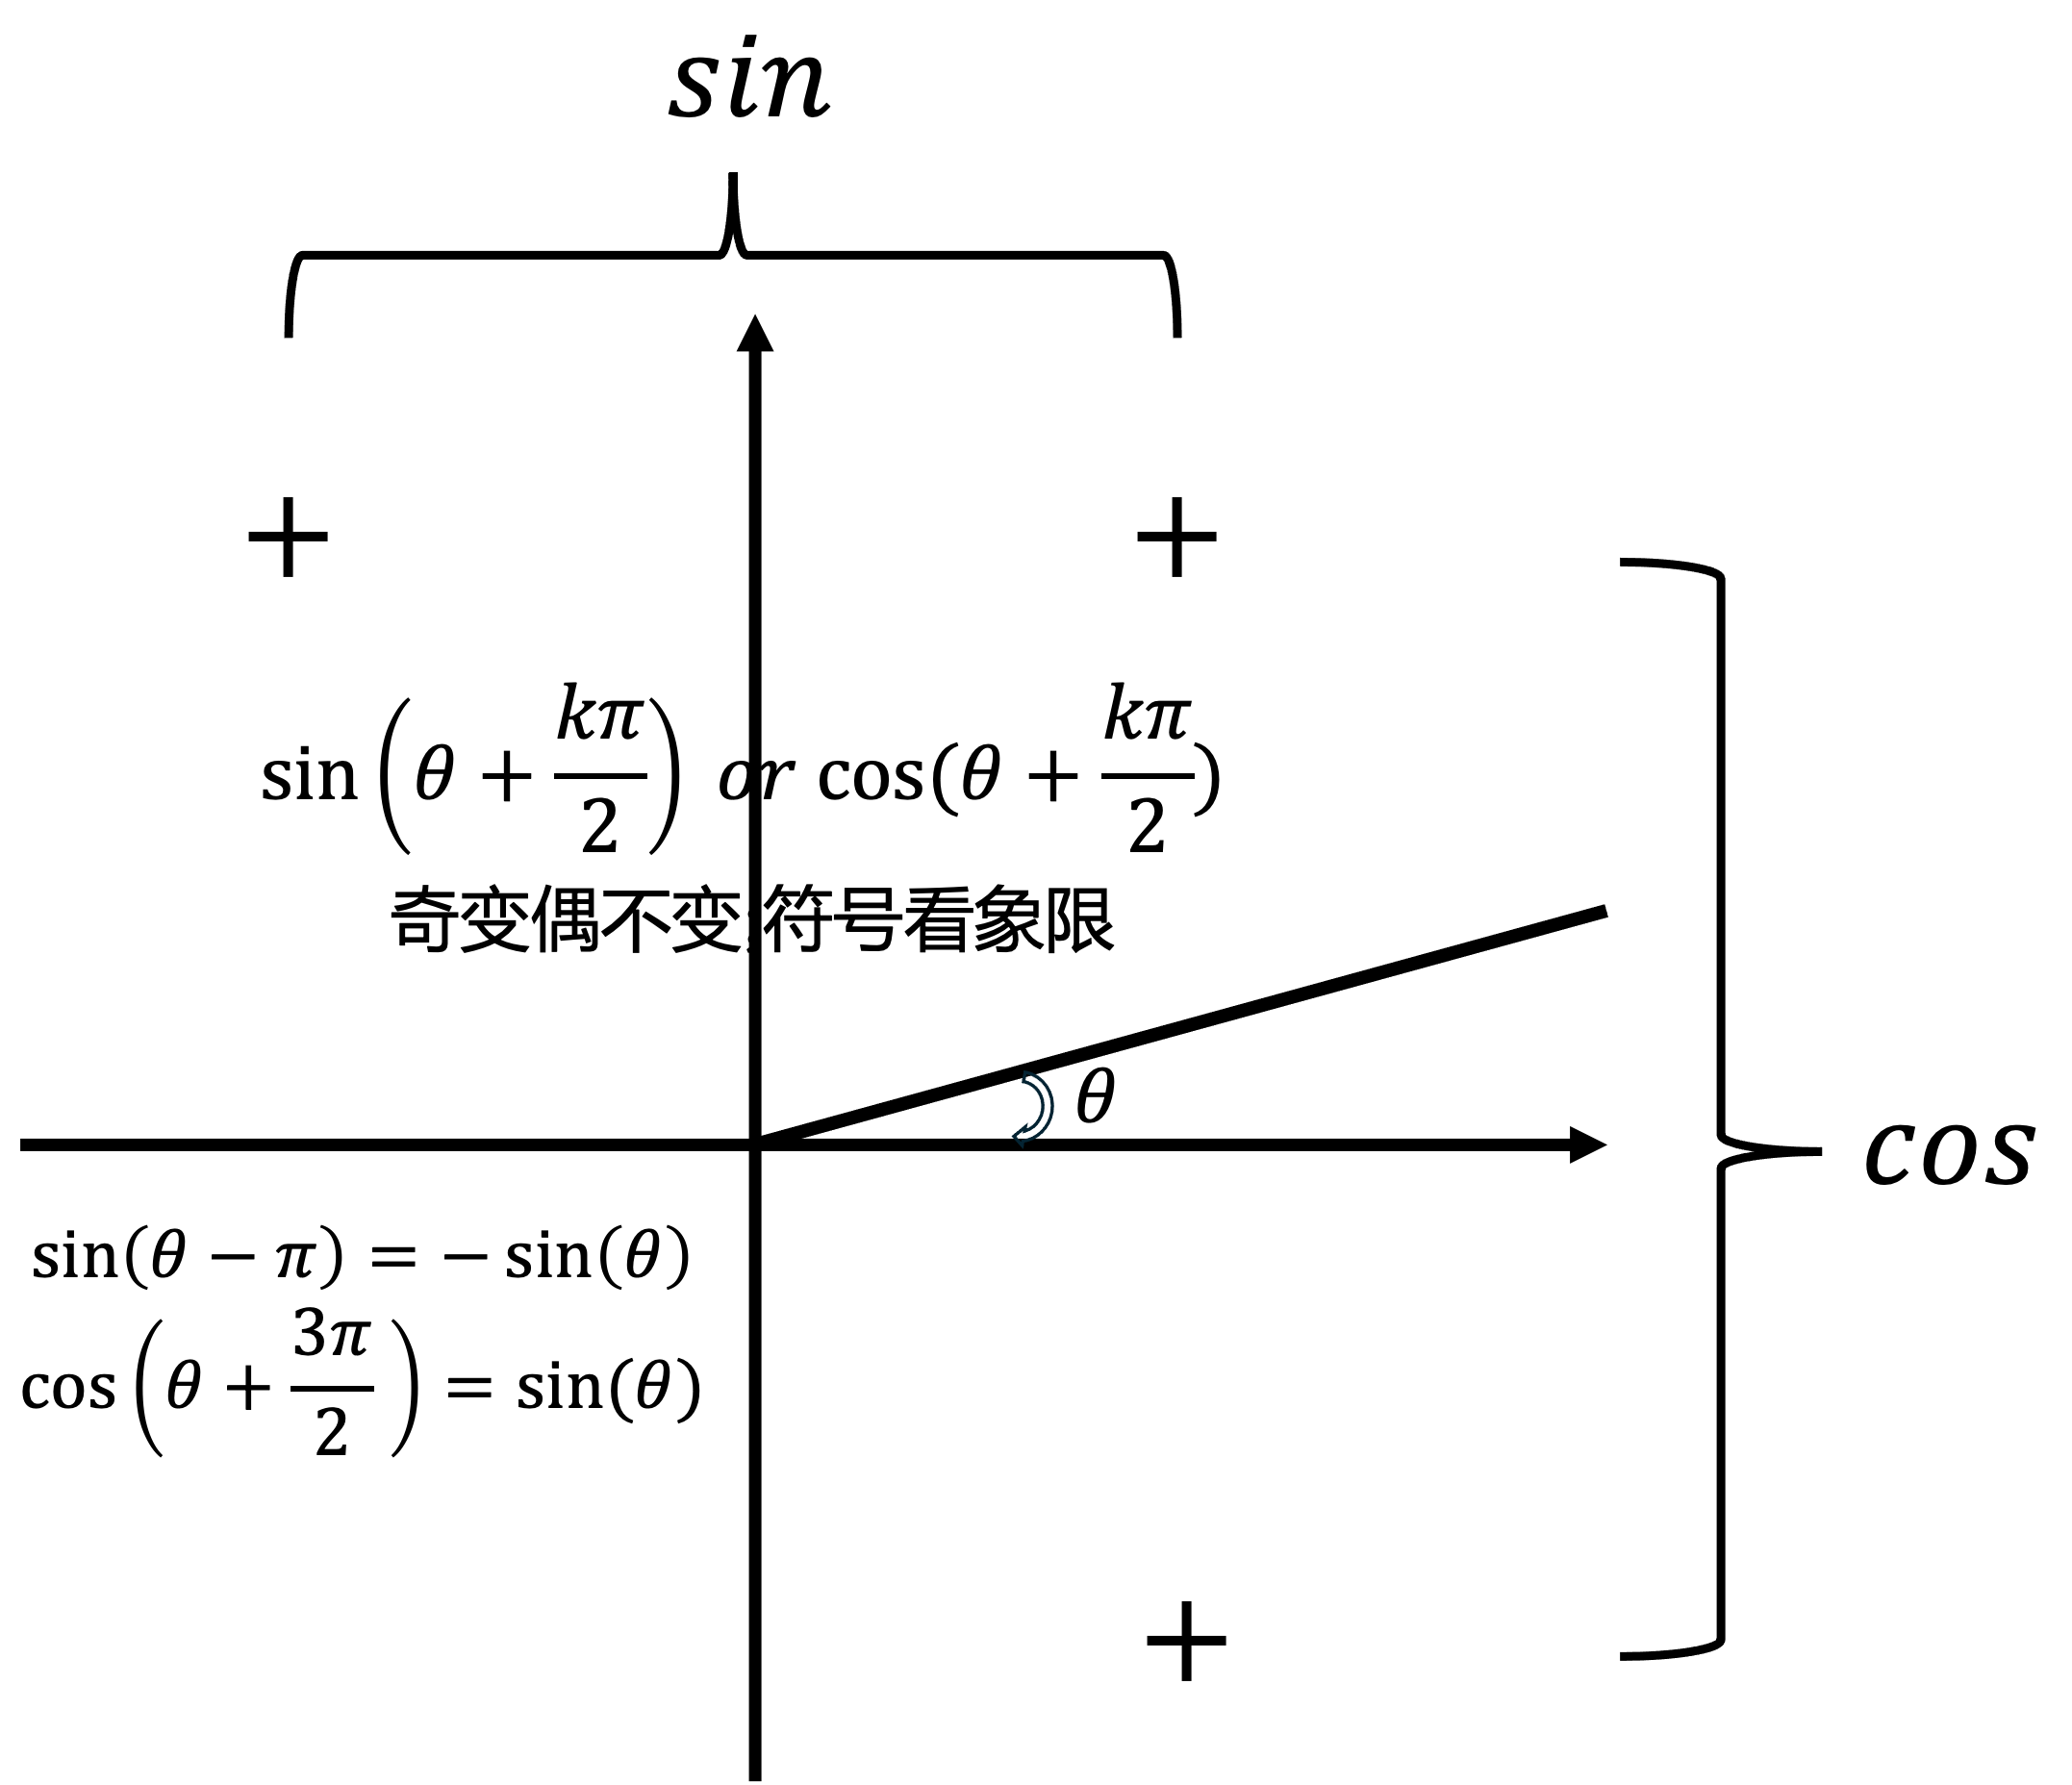
\includegraphics[width = 20em]{./pictures/1.png}

        \item 和关系
              $$ \sin^{2}{\theta}+\cos^{2}{\theta} = 1$$

        \item 正弦定理
              $$ \dfrac{a}{\sin{\alpha}} = \dfrac{b}{\sin{\beta}} = \dfrac{c}{\sin{\gamma}}   $$

        \item 余弦定理
              $$ \cos{\gamma} = \dfrac{a^{2}+b^{2} - c^{2}}{2ab} $$

        \item 二倍角
              $$ \sin{2\theta} = 2\sin{\theta}\cos{\theta} \quad \cos{2\theta} = \cos^{2}{\theta} - \sin^{2}{\theta} \quad \tan{2\theta} = \dfrac{2\tan{\theta}}{1-\tan^{2}{\theta}}$$

        \item 降次
              $$ \sin^{2}{\theta} = \dfrac{1 - \cos{2\theta}}{2} \quad \cos^{2}{\theta} = \dfrac{1 + \cos{2\theta}}{2} \quad \tan^{2}{\theta} = \dfrac{1-\cos{2\theta}}{1+\cos{2\theta}}$$
    \end{itemize}
\end{formal}

\vspace{2em}

\vspace{2em}

\section{光学}
\subsection{折射率}

\begin{itemize}
    \item 定义式:
          $$
              n = \dfrac{\sin{\text{大角}}}{\sin{\text{小角}}}
          $$
    \item 决定式:
          $$
              n = \dfrac{c}{v}
          $$
    \item 全反射:
          \begin{align*}
               & \text{光密介质} \, \ra \, \text{光疏介质} \quad \sin{\text{大角}} = 1 \,(\text{大角} = \frac{\pi}{2}) \\
               & \text{临界角} \quad \sin{C} = \frac{1}{\sin{\text{小角}}}
          \end{align*}
    \item 视深与视高:
          \begin{itemize}
              \item[] $H$为物点距离界面的高度;\,$h$为像点距离界面的高度
              \item 视深: \quad
                    从介质外看向介质内 \quad $h = \frac{1}{n} H$
              \item 视高: \quad
                    从介质内看向介质外 \quad $ h = n H $
          \end{itemize}
    \item 实验误差分析:
          \begin{itemize}
              \item 非平行玻璃砖 $\quad n_{\text{测}} = n_{\text{真}}$
              \item 整体平移  $\quad d_{\text{测}} = d_{\text{玻}} \quad n_{\text{测}} = n_{\text{真}}$
              \item 其他情况  $\quad n_{\text{测}} \text{和} n_{\text{真}} \text{的大小关系} \,\text{与}\, d_{\text{测}} \text{和} d_{\text{玻}}\text{的大小关系相反}$
          \end{itemize}
\end{itemize}

\vspace{2em}

\subsection{干涉实验}
\begin{enumerate}[label = (\arabic*{})]
    \item 薄膜干涉: $\delta = 2d$
          \begin{itemize}
              \item 明暗条纹位置由波长和此处厚度共同决定
              \item 相邻明(暗)条纹对应的薄膜厚度差为$\frac{\lambda}{2} \quad \lambda$应为光在介质中传播时的波长
          \end{itemize}
    \item 劈尖干涉: 样板下表面和被检查平面的上表面的反射光发生干涉

          \hspace{5em}(标准板的厚度太厚大于相干长度)

          \begin{itemize}
              \item[I] 验平问题:
                  \begin{itemize}
                      \item[] 若待测板平整,干涉条纹等距
                      \item[] 若条纹\textbf{偏头},则条纹提前出现,此处光程差偏大,因此待测样板此处凹
                      \item[] 若条纹\textbf{偏尾},则条纹延后,此处光程差偏小,因此待测样板此处凸
                  \end{itemize}
              \item[II] 条纹间距问题:
                  \begin{itemize}
                      \item[] 薄片(支撑两个板)的移动改变$\theta$角 $\quad \triangle l = \dfrac{\triangle d}{\tan{\theta}} \quad
                              \triangle d = f(\lambda) = \dfrac{\lambda}{2}$
                  \end{itemize}
              \item[III] 增反膜;增透膜: 入射光能量 = 折射光能量 + 反射光能量

                  \hspace{4em}(注:光疏到光密反射光产生半波损失,$n_{\text{膜}}$介于空气和另一介质之间)

                  \hspace{4em}增透膜:反射光相消$2d = \frac{\lambda}{2} (2n+1)$

                  \hspace{4em}增反膜:反射光相长$2d = \frac{\lambda}{2} (2n) $
          \end{itemize}

    \item 双缝干涉: $\triangle d = \lambda \dfrac{L}{d} \,$ (条纹间距$\triangle d $,双缝间距$d$,缝板距离$L$)
\end{enumerate}

\vspace{2em}

\subsection{总结}
\begin{formal}
    符号说明

    \vspace{0.5em}

    \begin{tabular}{|c|c|c|c|c|c|c|c|c|c|}
        \hline
        频率  & 折射率 & 速度  & 临界角 & 波长        & 动量  & 干涉            & 能量            & 逸出功     & 逃逸光子动能  \\
        \hline
        $f$ & $n$ & $v$ & $C$ & $\lambda$ & $p$ & $\triangle x$ & $\varepsilon$ & $w_{0}$ & $E_{k}$ \\
        \hline
    \end{tabular}

    \vspace*{2em}

    \begin{itemize}
        \item 同一介质中不同频率的光

              \vspace*{1em}
              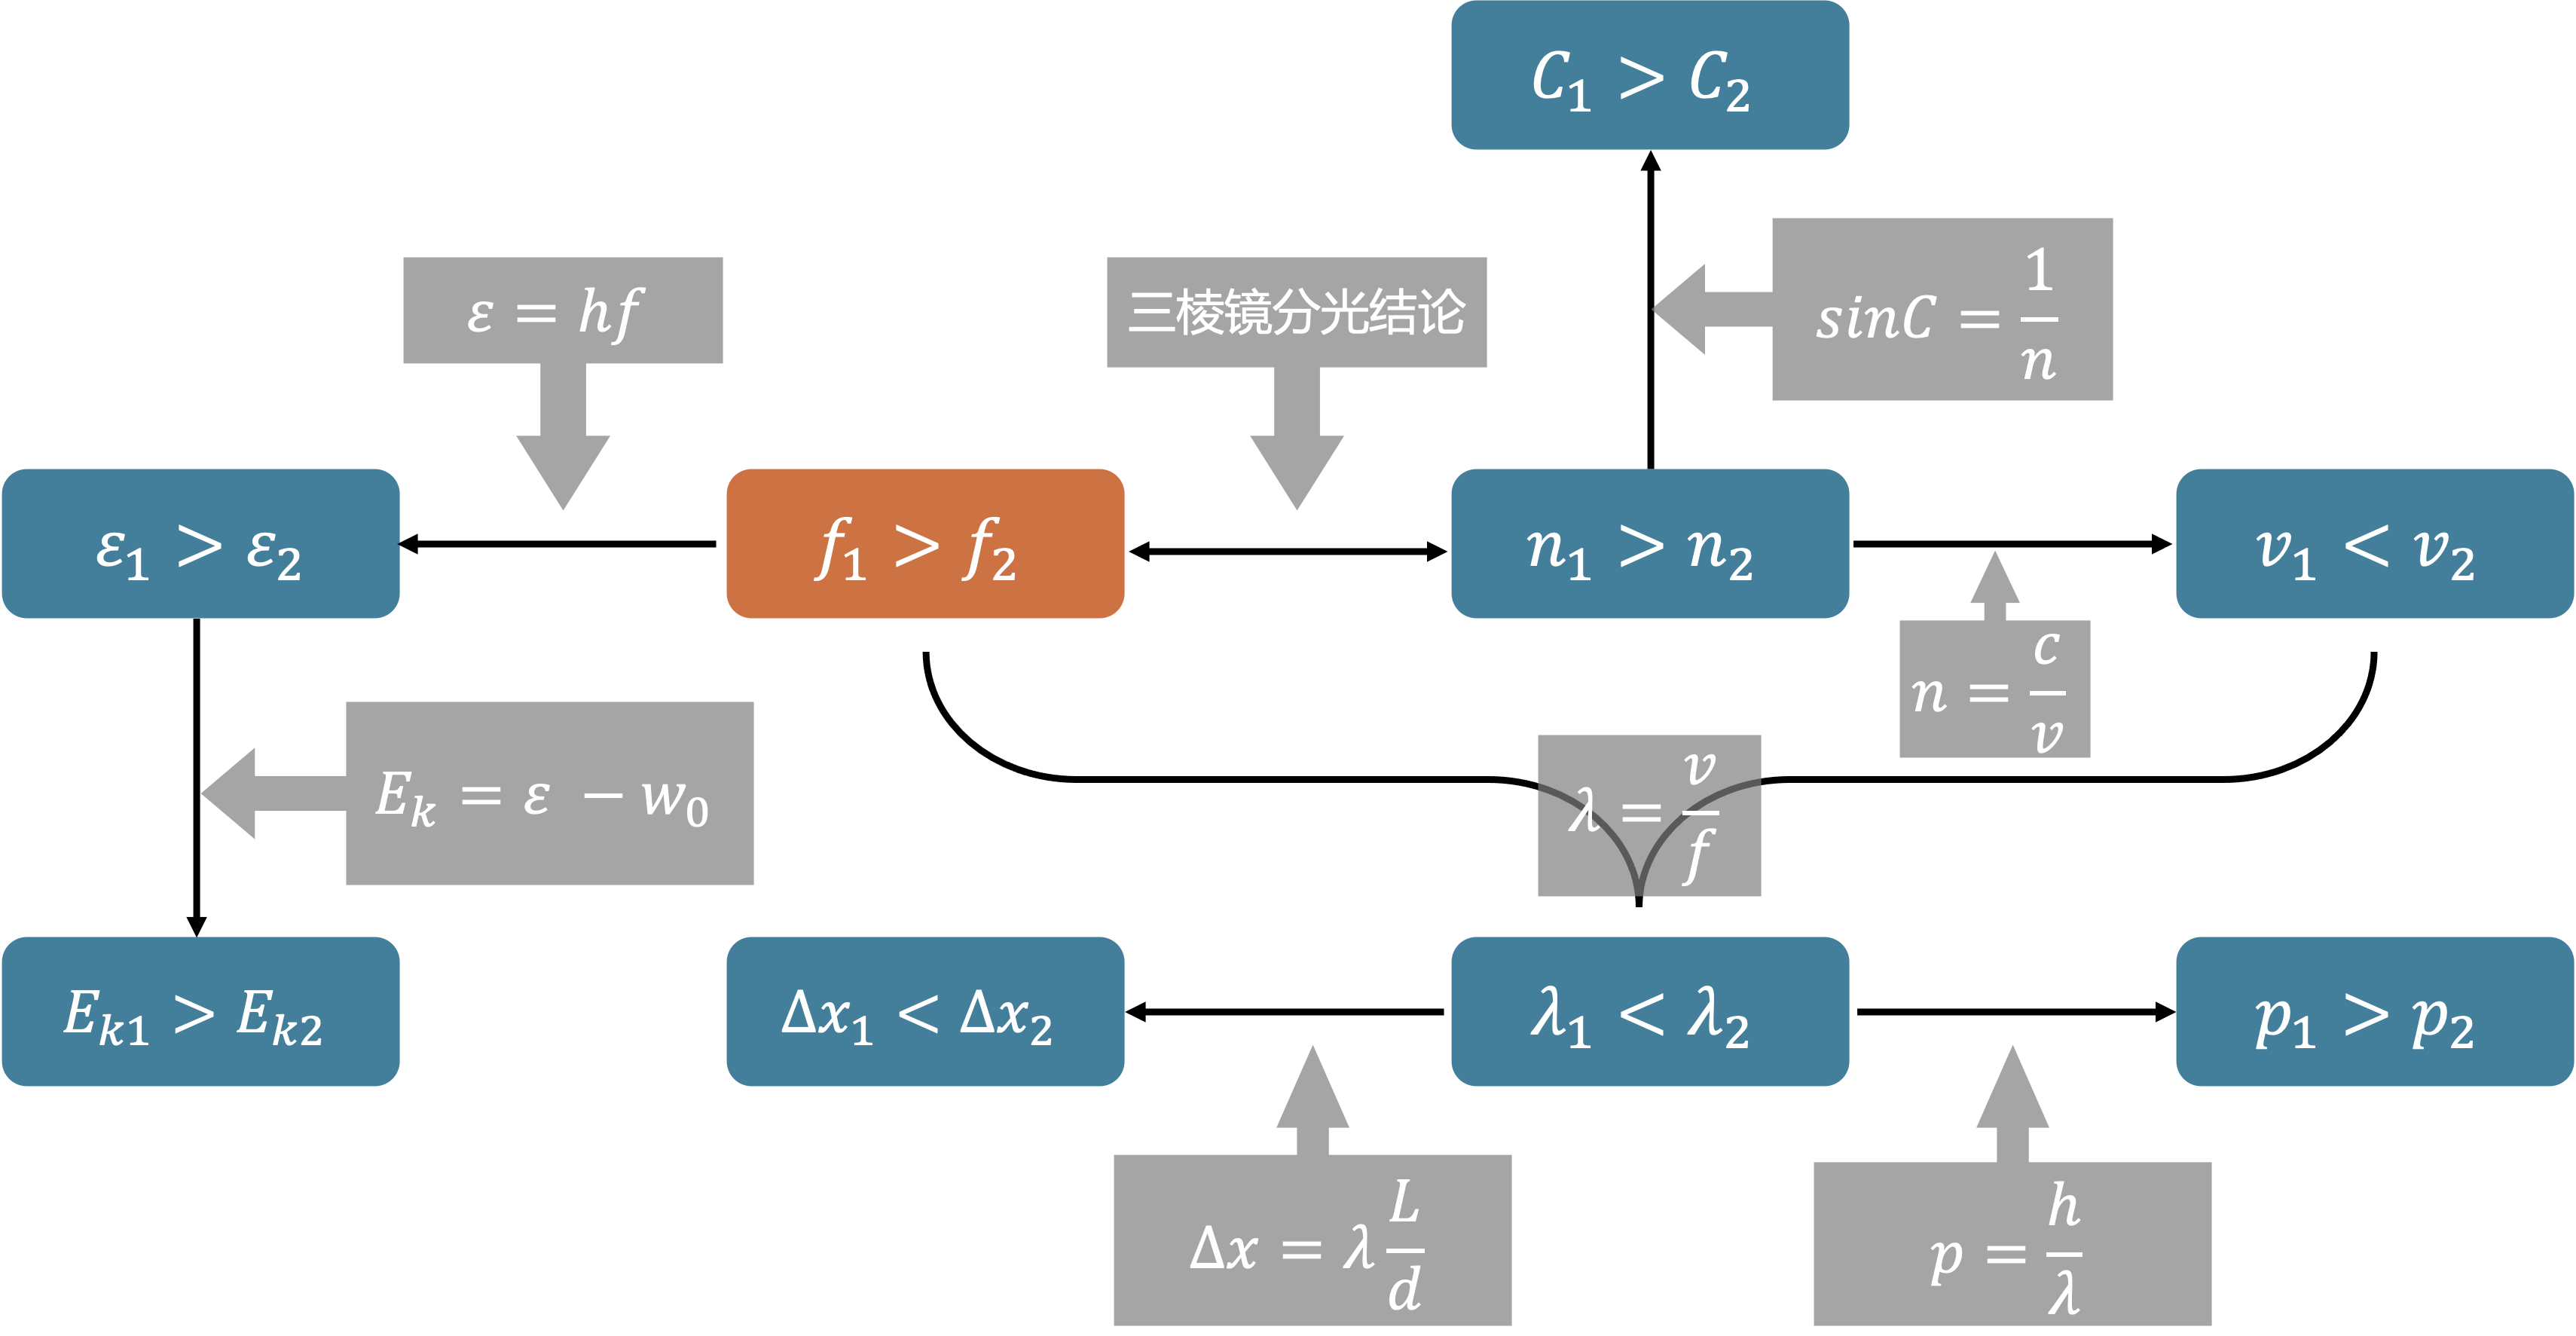
\includegraphics[width=35em,keepaspectratio]{./pictures/2.png}

              \vspace*{2em}

        \item 同一频率的光在不同介质(下标表示不同介质中)中

              \vspace*{1em}
              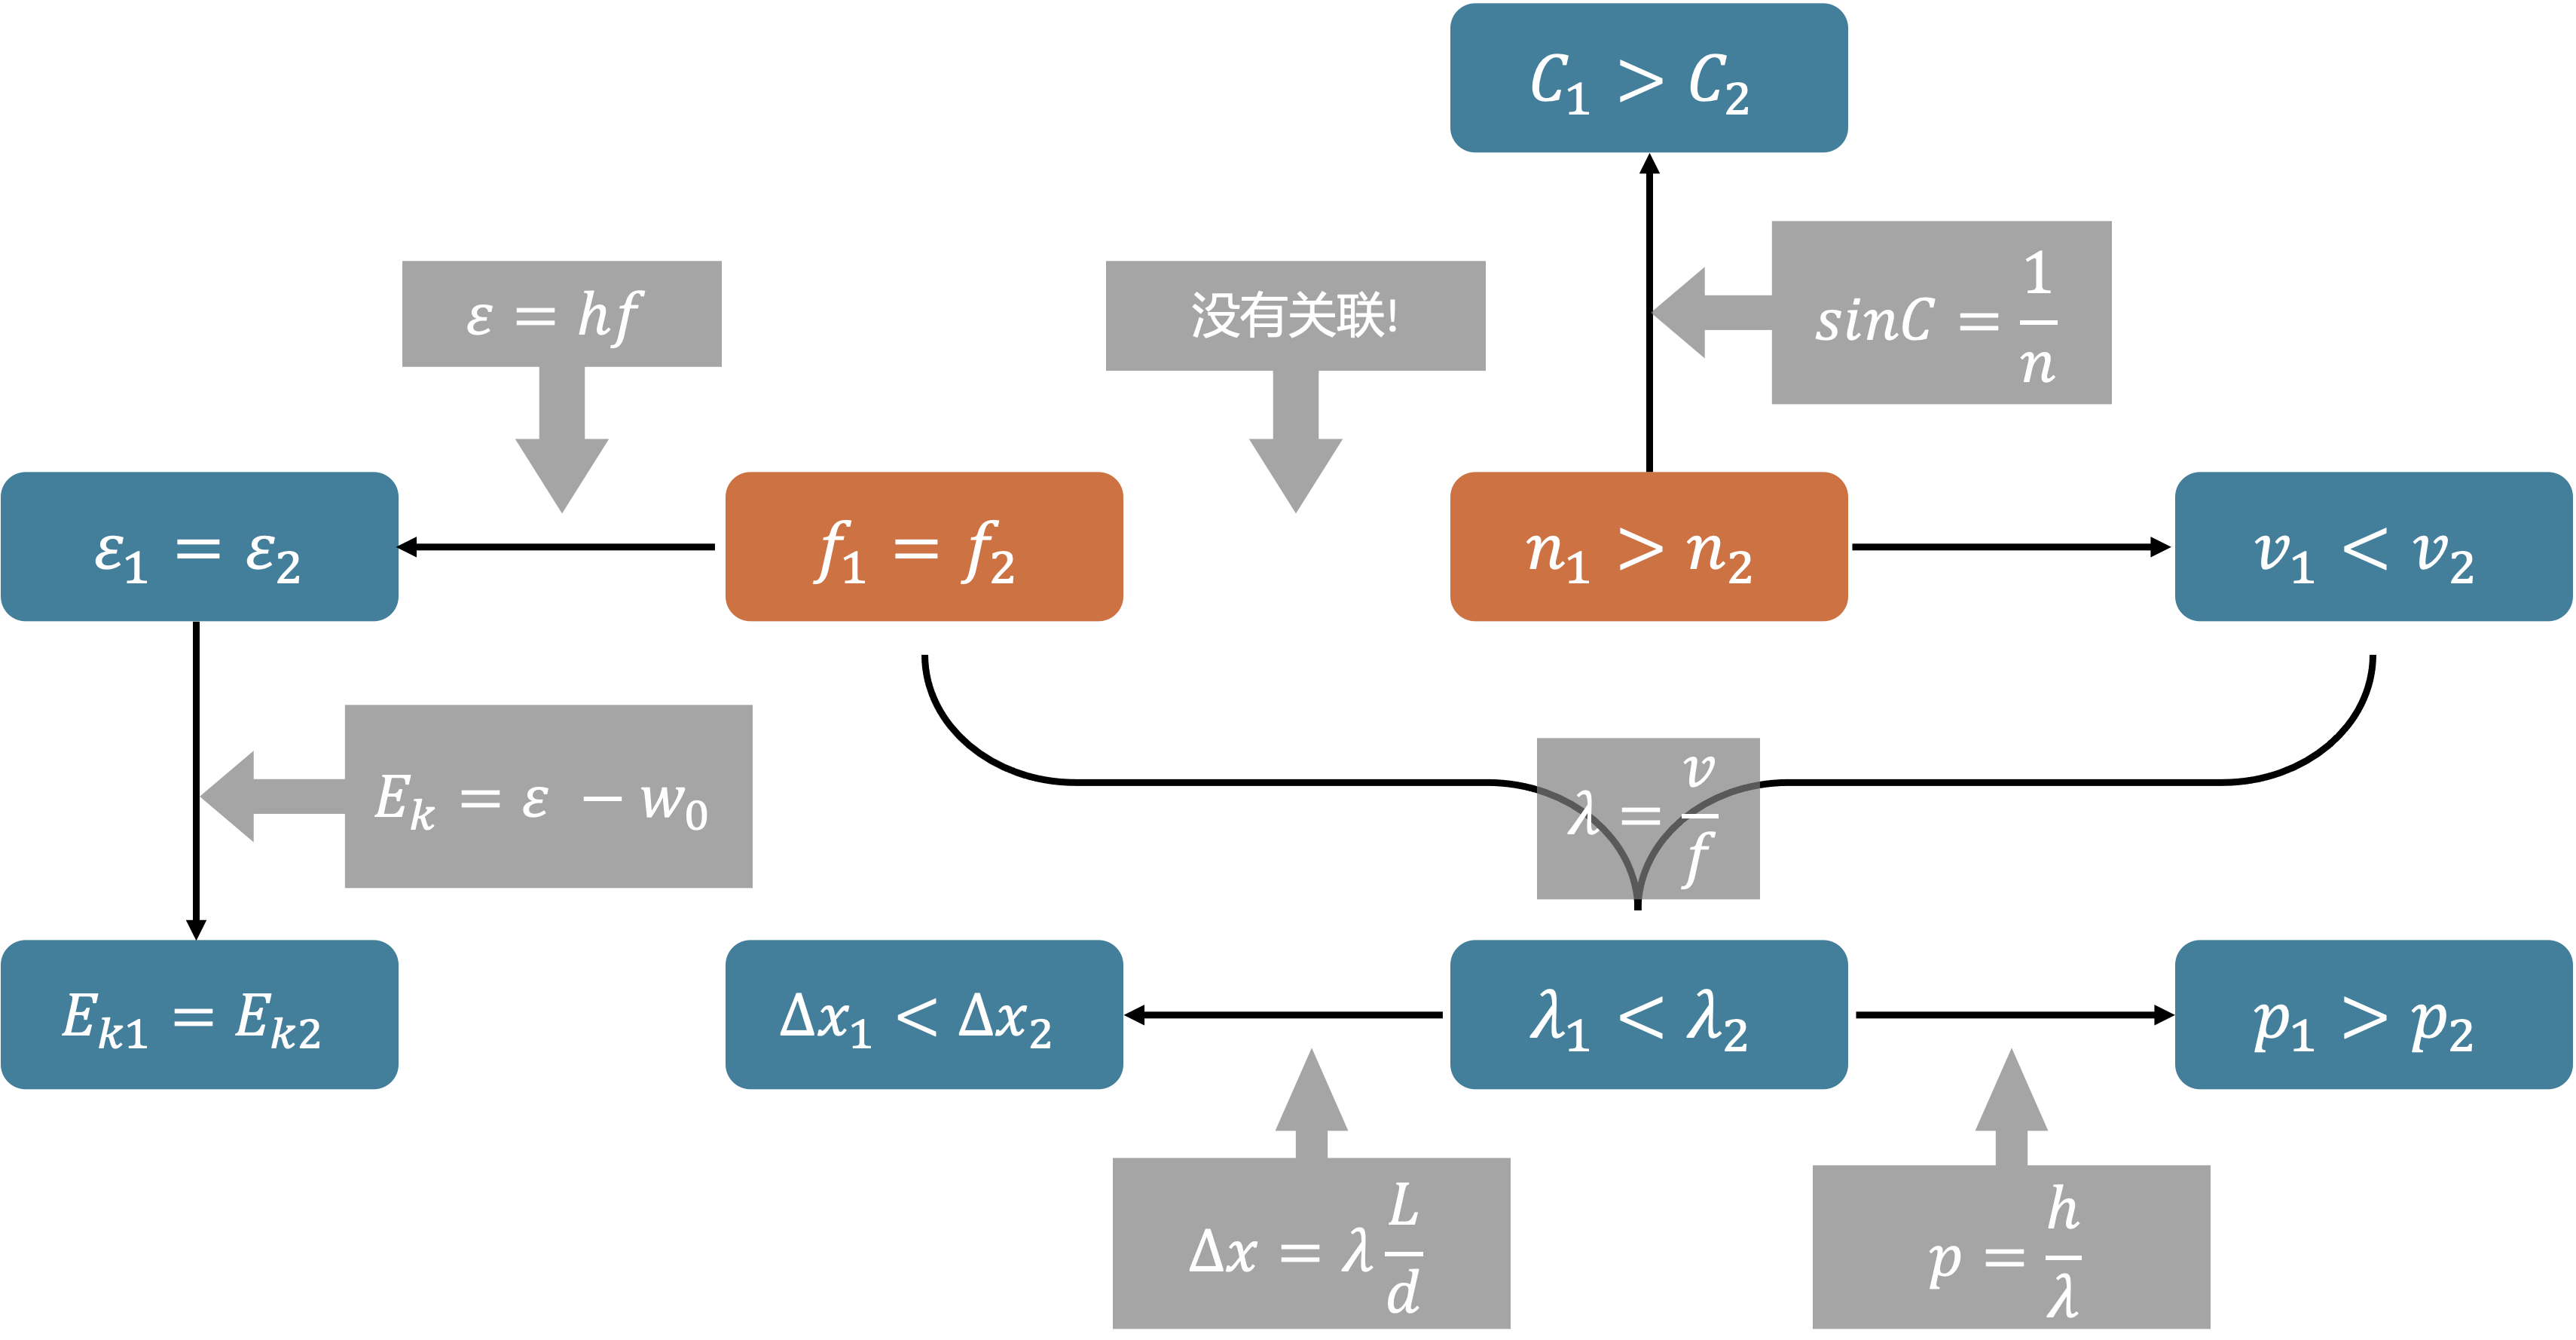
\includegraphics[width=35em,keepaspectratio]{./pictures/3.png}
    \end{itemize}
\end{formal}

\vspace{2em}

\section{热力学}
\subsection{分子动理论}
\subsubsection{物体是由大量分子构成的}
\begin{enumerate}
    \item 分子的大小
          \begin{enumerate}[label = (\arabic*{})]
              \item 分子直径数量级: $10^{-10} \, m$
              \item 分子质量数量级: $10^{-26} \, kg$
              \item 测量分子的方法: 油膜法
          \end{enumerate}

          \vspace{2em}

    \item 两种分子模型
          \begin{enumerate}[label = (\arabic*{})]
              \item 球体模型: 认为分子是一个个紧挨着的球体(适用对象: 固体,液体;体积:$V = \frac{4\pi}{3} R^{3}$)
              \item 立方体模型: 认为分子是一个个紧挨着的立方体(适用对象: 气体;体积:$V = d^{3}$)
          \end{enumerate}

          \vspace{-1em}
          \begin{adjustbox}{minipage=0.86\linewidth, bgcolor=gray!20, padding=1em}
              \small
              固液相使用球体模型更为准确,气相使用立方体模型更为准确,这里的立方体空间是气体分子的活动空间
          \end{adjustbox}
          \vspace{-1em}

          \vspace{2em}

    \item 油墨法测量分子的直径
          \begin{itemize}
              \item 思路: 第一滴油酸摊开在水面上,近似看成单分子层
              \item 模型: 认为油酸分子为球体模型
              \item 要点:
                    \begin{itemize}
                        \item $1ml$油酸溶液配制成$500ml$油酸酒精溶液
                        \item 取$100$滴油酸酒精溶液测得体积为$1ml$
                        \item 先对水撒痱子粉,后滴液解决油膜的透明问题
                        \item 往水面上注射一滴油酸酒精溶液
                        \item 稳定后使用玻璃板盖进行描边
                        \item 使用\textbf{格子法}来计算不规则面积(不足半格取$0$,超过半格取$1$)
                    \end{itemize}
          \end{itemize}

          \vspace{2em}

          \subsubsection{微观量的估算}
          \begin{enumerate}[label = (\arabic*{})]
              \item 分子层面: 单个分子质量$m_{0}$,单个分子所占空间体积$V_{0}$
              \item 化学层面: 摩尔质量$M_{mol} \, (g \slash mol)$,摩尔体积$V_{mol} \, (L \slash mol)$
              \item 实际层面: 质量$M$,体积$V$
              \item[] 物理量之间的关系: $n = \frac{N}{N_{A}} \, mol \, (N_{A} = 6.02 \cross 10^{23})$
                  $$
                      M_{mol} = \frac{M}{n}   \quad   m_{0} N_{A} = M_{mol}
                  $$
                  $$
                      V_{mol} = \frac{V}{n}   \quad   V_{0} N_{A} = V_{mol} \quad
                  $$
                  $$
                      \hspace{0.2em} \text{摩尔体积适用于固液相,但是计算出来的并不能视作单分子体积,而是单分子占用空间}
                  $$
                  $$
                      \text{摩尔体积不适用于气体,因为标况下气体为}22.4L\text{,那么除以}N_{A}\text{会导致每个分子一样大}
                  $$

                  \vspace{-1em}
                  \hspace{-1em}
                  \begin{adjustbox}{minipage=0.38\linewidth, bgcolor=gray!20, padding=1em}
                      \small % 将字号变小为 small
                      标况: $0^{\circ}C$,一个标准大气压(约$101kPa$)
                  \end{adjustbox}

              \item[] 密度: 区分 \, 分子密度 \, 与 \, 气体密度,利用气体密度所求体积为 \,分子所占空间体积
          \end{enumerate}

\end{enumerate}

\vspace{2em}

\subsubsection{扩散现象和布朗运动}
一切物质的分子都在不停地做无规则的(热)运动

\begin{enumerate}
    \item 扩散现象
          \begin{enumerate}[label = (\arabic*)]
              \item 定义: 相互接触的不同物质能够彼此进入对方

                    \hspace{2.7em}此现象并不是宏观受力的作用下发生的,且各个状态下都会存在扩散现象
              \item 前提: 浓度差(梯度)
              \item \textbf{直接}反映了分子的无规则运动
              \item 扩散现象的快慢: 与物质的状态与温度有关,气体$>$液体$>$固体
          \end{enumerate}
    \item 布朗运动
          \begin{enumerate}[label = (\arabic*)]
              \item 定义: 悬浮在液体或(气体)中的微粒(宏观层面)的无规则运动
              \item 实验背景: 布朗看水中的花粉(显微镜)
              \item 观察结论: 微粒越小或温度越高,布朗运动越强烈
              \item 原因: 水分子对布朗微粒撞击的不平衡(不均匀)
              \item 布朗运动\textbf{不是}分子运动,\textbf{间接}反映了分子的无规则运动
          \end{enumerate}
    \item 扩散与布朗运动的混淆点
          \begin{enumerate}[label = (\arabic*)]
              \item 扩散现象: 微观力作用,宏观现象肉眼可见
              \item 布朗运动: 宏观力作用,宏观现象光学显微镜观察可见($10^{-6}$)
              \item 两者都是微观层面的分子无规则运动所形成的宏观现象
          \end{enumerate}
\end{enumerate}

\vspace{2em}

\subsubsection{分子之间的作用力}
\begin{itemize}
    \item 现象
          \begin{enumerate}[label = (\arabic*)]
              \item 分子虽然有空隙,大量分子聚集形成固体或液体说明了分子之间存在\textbf{引力}
              \item 用力压缩物体,物体内会产生反抗压缩的弹力,说明了分子之间存在斥力
          \end{enumerate}
    \item 研究表明
          \begin{enumerate}[label = (\arabic*)]
              \item 分子之间引力和斥力\textbf{同时存在}
              \item 引力与斥力都随着分子间距离增大而减小
              \item 斥力的变化比引力的变化更加明显
          \end{enumerate}
    \item 结论
          \begin{enumerate}[label = (\arabic*)]
              \item 分子距离较近时$<r_{0}$体现为 \, \textbf{斥力}
              \item 分子距离较远时$>r_{0}$体现为 \, \textbf{引力}
              \item 分子距离为$=r_{0}$合力为$0$
              \item 当分子间距离$>10 \, r_{0}$,引力、斥力均忽略不计
          \end{enumerate}

\end{itemize}

\vspace{2em}

\subsubsection{分子之间的能量}
\begin{itemize}
    \item 分离两个很近的分子
          \begin{enumerate}[label = (\arabic*)]
              \item 做功情况: 先斥力做正功,后续引力做负功
              \item 能量变化: 分子势能先减小,后增大
              \item 默认规定: 取无穷远处地方的势能为$0$
              \item 特殊点: $d = r_{0}$时,合力最小,势能最小(且为负)
          \end{enumerate}
    \item 分子势能的体现
          \begin{enumerate}[label = (\arabic*)]
              \item 微观上: 分子势能与分子间位置有关
              \item 宏观上: 分子势能与宏观体积有关
          \end{enumerate}
\end{itemize}

\vspace{2em}

\subsubsection{分子动能}
\begin{itemize}
    \item 分子动能
          \begin{enumerate}[label = (\arabic*)]
              \item 定义: 分子热运动所具有的能量
              \item 分子平均动能: 所有分子动能的平均值
              \item 研究单个分子的动能没有意义,所以我们研究的动能是分子的平均动能
              \item 影响因素: 有且只有一个\textbf{温度}
              \item 易错点: 平均分子动能与分子种类无关,与实际速度无关

                    \hspace{3.7em}单个分子的动能与温度并非严格正相关
          \end{enumerate}
    \item 分子势能的体现
          \begin{enumerate}[label = (\arabic*)]
              \item 微观上: 分子势能与分子间位置有关
              \item 宏观上: 分子势能与宏观体积有关
          \end{enumerate}
    \item 图像中分子动能的规律

          \vspace{-1em}
          \begin{adjustbox}{minipage=0.91\linewidth, bgcolor=gray!20, padding=1em}
              \small % 将字号变小为 small
              $$ f(v)= \frac{dN}{Ndv} ={\sqrt {{\frac {2}{\pi }}\left({\frac {m}{kT}}\right)^{3}}}\,v^{2}\exp \left({\frac {-mv^{2}}{2kT}}\right)  \quad
                  \int_{0}^{+\infty} f(v) dv  = \int_{0}^{N} \frac{dN}{N} = 1
              $$
              $$
                  [v_{1},v_{2}] \, \text{区间分子数} N_{0} = \int_{v_{1}}^{v_{2}} N f(v) dv  \quad [v_{1},v_{2}] \, \text{区间的概率} \frac{dN}{N} = \int_{v_{1}}^{v_{2}} f(v) dv
              $$
          \end{adjustbox}
          \vspace{-1em}

          \begin{minipage}{0.45\textwidth}
              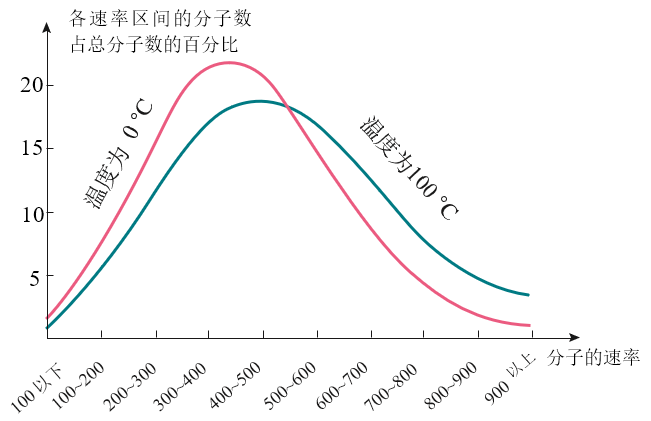
\includegraphics[width=\textwidth,keepaspectratio]{./pictures/23.png}
          \end{minipage}
          \hfill
          \begin{minipage}{0.45\textwidth}
              \begin{enumerate}[label = (\arabic*)]
                  \item 中间高,两头低
                  \item[]
                  \item 温度越高,峰值点下降并横移
                  \item[]
                  \item 任何温度下,图像围成的面积为$1$
              \end{enumerate}
          \end{minipage}
\end{itemize}

\vspace{2em}

\subsubsection{温度和温标}
\begin{enumerate}
    \item 气体的状态参量
          \begin{itemize}
              \item 几何性质: 体积
              \item 力学性质: 压强
              \item 热学性质: 温度
              \item $\dfrac{PV}{T} = C \,$ ($C$常数,与质量和气体种类相关)
          \end{itemize}
    \item 温度
          \begin{itemize}
              \item 意义: 宏观上表示物体的冷热程度,微观上表示的是分子热运动的剧烈程度
              \item 温标: 摄氏温度$t \, ^{\circ}$,热力学温标$T$,单位$K$(开)
              \item 转化: $T = t + 273.15 \,$(绝对零度: $T = 0 \lra t = -273.15^{\circ} $)
          \end{itemize}
    \item 热平衡: 两个热力学系统之间无温度差(温度相同)
\end{enumerate}

\vspace{2em}

\subsubsection{内能}
\begin{enumerate}
    \item 分子势能: 由分子的\textbf{位置}决定,在微观上与\textbf{分子间距}相关,宏观上与\textbf{体积}相关
    \item 内能的概念: 物体\textbf{所有分子}的 热运动的动能与分子势能的总和
    \item 内能的决定因素:
          \begin{enumerate}[label = (\arabic*)]
              \item 微观上: 分子个数,分子平均动能,分子势能
              \item 宏观上: 质量,温度,体积
          \end{enumerate}
    \item 分子平均动能: 温度
    \item 理想气体: 有质量,分子无体积,分子之间没有作用力的气体
    \item 两个意义: 分子无体积(仍有占有体积)意味着气体可以无限被压缩

          \hspace{4.7em}分子间无作用力(气体内能不包含势能)
    \item 结论: 理想气体内能只有动能项,其内能大小仅和温度有关
\end{enumerate}

\vspace{2em}

\subsection{物态及物态的变化}
\subsubsection{晶体与非晶体}
\begin{enumerate}
    \item 固体
          \begin{itemize}
              \item 根据有无固定熔点分为: 晶体(有) \, 非晶体(无)
              \item 根据有无规则的外形分为: 单晶体(有) \, 多晶体(无)

                    \vspace{-1em}
                    \begin{adjustbox}{minipage=0.76\linewidth, bgcolor=gray!20, padding=1em}
                        \small % 将字号变小为 small
                        单晶体: 其内部微粒有规律地排列在一个空间格子内的晶体.

                        \hspace{3.8em}其晶体结构是连续的,或者可以说,在宏观尺度范围内单晶不包含晶界.

                        \,

                        多晶体: 仅存在于固体,由多颗大小及方向各异的晶粒所构成

                        \hspace{3.8em}而这些晶粒一般都由大量微小的单晶或微晶(微结晶、结晶粒、结晶子)组成.

                        \hspace{3.8em}在材料不同位置生长的结晶粒相遇时形成晶界
                    \end{adjustbox}
                    \vspace{-1em}

              \item 常见晶体: 石英 \, 食盐 \, 明矾 \, 云母 \, 天然水晶
              \item 常见非晶体: 蜂蜡 \, 橡浆 \, 玻璃
              \item 互相转换:

                    \hspace{4.8em}糖块 \, 是多晶体;组成糖块的颗粒 \, 是单晶体

                    \hspace{4.8em}天然水晶 \, 是单晶体;融化后再凝固的玻璃 \, 是非晶体
          \end{itemize}

    \item 各向同性与各向异性:
          \begin{itemize}
              \item 定义: 各个方向上的物理性质的同异(主要指导电性,导热性,透光性等)
              \item 单晶体: 其具有规则外形,因此不同方向上物理性质具有差异,各向异性
              \item 多晶体与非晶体: 其具有不规则外形,因此不同方向上物理性质一致,各向同性
          \end{itemize}

    \item 总结:

          \hspace{3em}\begin{tabular}{|c|c|c|c|}
              \hline
                   & 单晶体  & 多晶体  & 非晶体  \\
              \hline
              外形   & 规则   & 无规则  & 无规则  \\
              \hline
              固定熔点 & 有    & 有    & 无    \\
              \hline
              物理性质 & 各向异性 & 各向同性 & 各向同性 \\
              \hline
          \end{tabular}
\end{enumerate}

\vspace{2em}

\subsubsection{液体}
\begin{enumerate}
    \item 表面张力
          \begin{enumerate}[label = (\arabic*)]
              \item 生活中的现象: 球形露珠,水面上的水蜘蛛
              \item 作用: 表面张力是的液体具有\textbf{收缩}的趋势
              \item 效果: 使得表面积趋于最小,而在体积$V$相同的情况下,\textbf{球体表面积最小}
              \item 成因: 表面层蒸发使得分子较为稀疏,间距较大,表现为分子间的引力
              \item 方向: 与液体表面相切,与液体的分界线垂直
              \item 大小: 温度越高张力越小(例如蒸发现象),有杂质的时候张力更小(类似隔断)
          \end{enumerate}
    \item 浸润与不浸润
          \begin{enumerate}[label = (\arabic*)]
              \item 浸润现象: 毛巾洗脸,下雨衣服湿了,试管凹液面
              \item 不浸润现象: 荷叶上的水滴,水银凸液面
              \item 成因: 固体分子对液体分子的作用力

                    \begin{center}
                        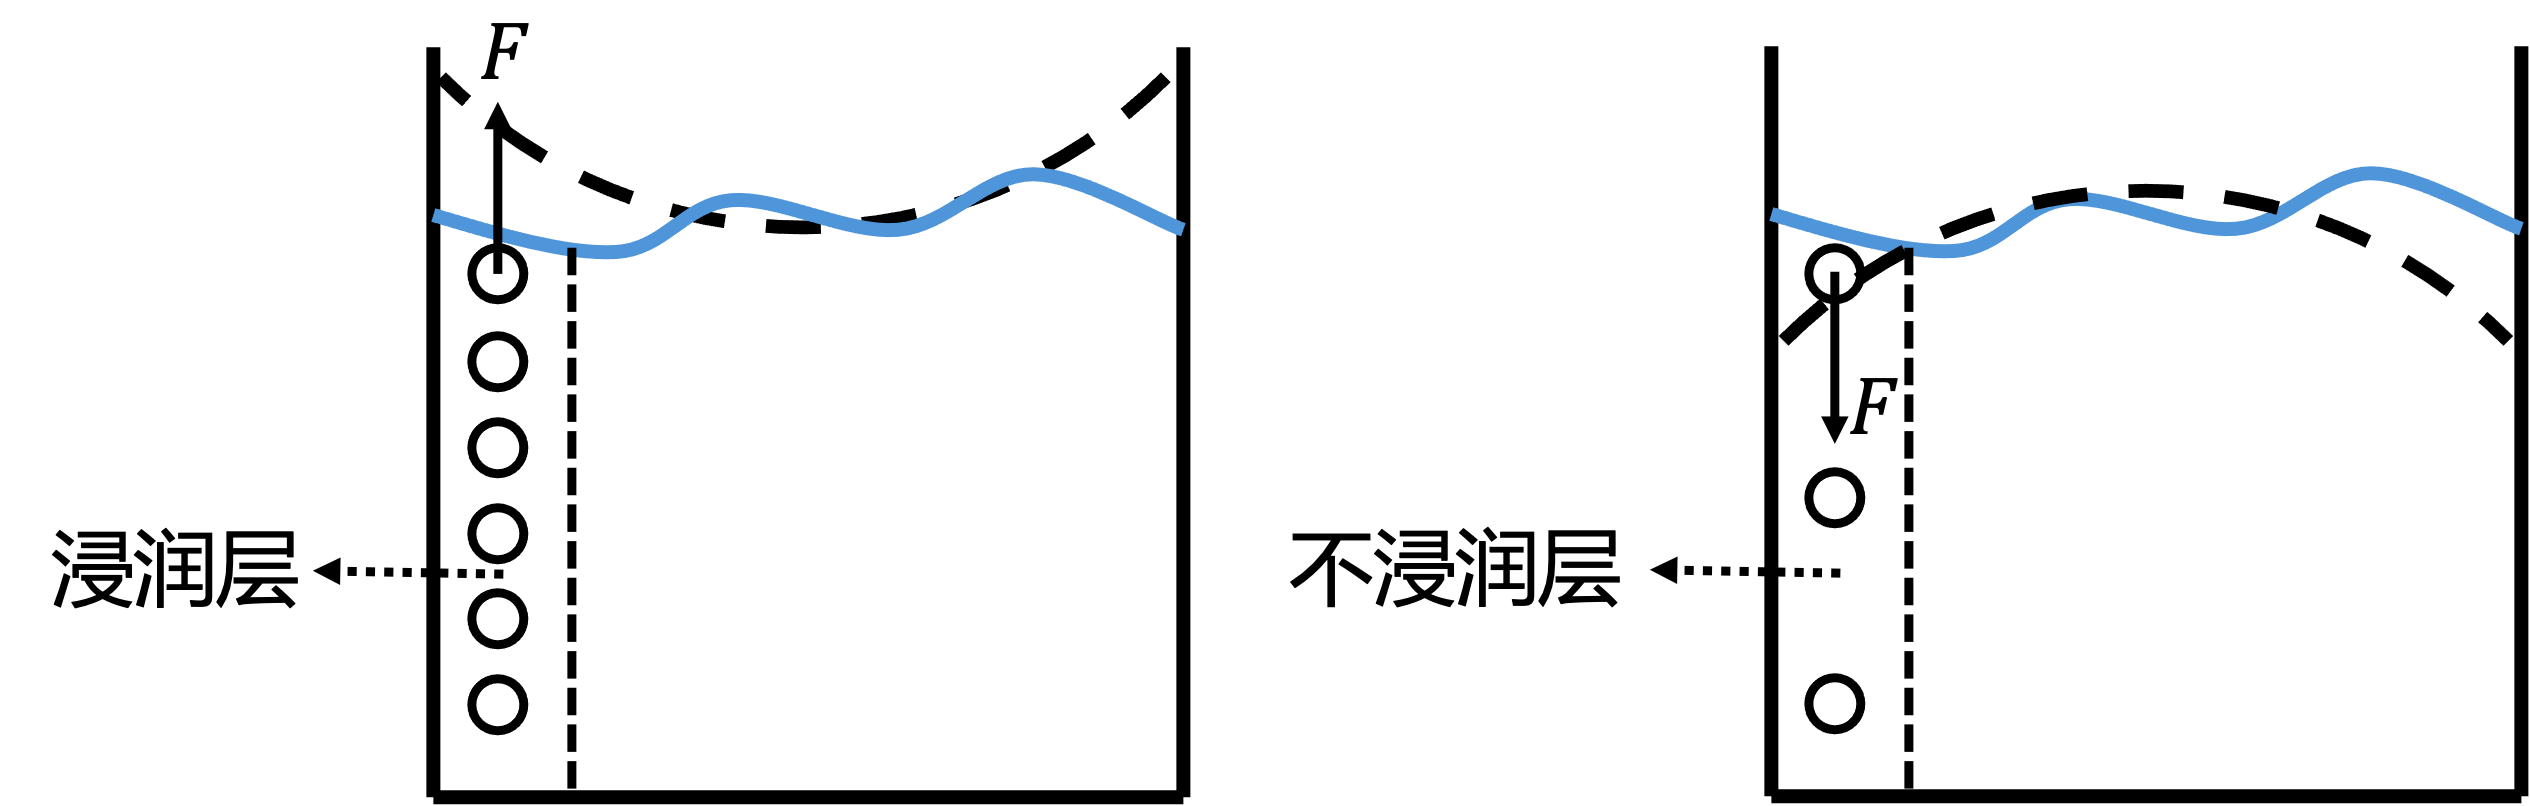
\includegraphics[width = 0.8\textwidth]{./pictures/24.png}
                    \end{center}

              \item 毛细现象: 本质上是 \, \textbf{浸润} \,和\, \textbf{表面张力} \, 的共同作用

                    \hspace{4.7em}\begin{minipage}{0.7\textwidth}
                        浸润时尽可能贴附固体分子(水液面上升)

                        非浸润时尽可能排斥固体分子(水银液面下降)

                        试管越细,那么管内的液体则越少,毛细现象越明显

                        \vspace{-1em}
                        \begin{adjustbox}{minipage=0.7\linewidth, bgcolor=gray!20, padding=1em}
                            \small 
                            液面上升高度 $\, h= \dfrac{2\gamma \cos{\theta}}{\rho gr} \quad $($\theta$:液面切线与固体面所成锐角)

                            $\gamma$:表面张力系数;$\quad \theta$:接触角;$\quad \rho$:液体密度;$\quad r$:试管半径
                        \end{adjustbox}
                        \vspace{-1em}

                        下雨\textbf{踩土}(减少土壤缝隙宽度)\textbf{加强}毛细现象,减少树木根部积水

                        下雨\textbf{刨土}(使得土壤不再有缝隙)\textbf{破坏}毛细现象,增加树木根部水量
                    \end{minipage}
          \end{enumerate}

    \item 液晶: 像液体一样具有流动性,光学性质与单晶体相似具有各向异性

          \hspace{2.4em} 液晶不是单/多晶体与非晶体,独立种类

          \begin{center}
              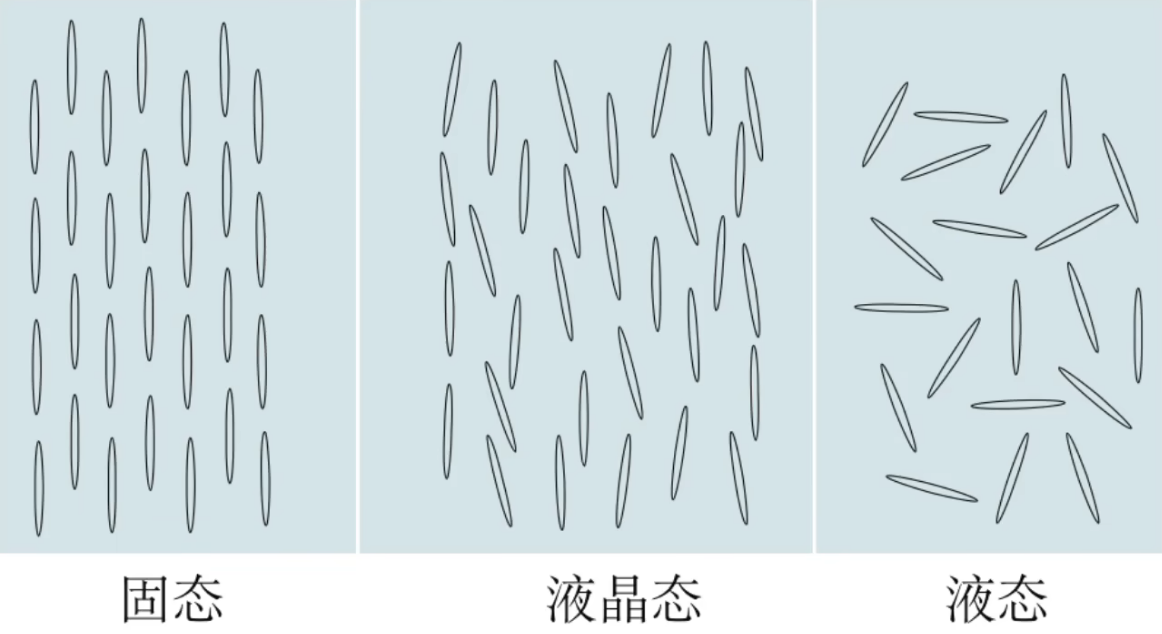
\includegraphics[width = 0.5\textwidth]{./pictures/25.png}
          \end{center}
\end{enumerate}

\vspace{2em}

\subsubsection{饱和汽与饱和汽压}
\begin{enumerate}
    \item 概念:
          \begin{enumerate}[label = (\arabic*)]
              \item 饱和汽: 与液体处于动态平衡的蒸汽
              \item 饱和汽压: 饱和汽的压强
          \end{enumerate}
    \item 理解: 在溶液中既有水分子蒸发出去,也有水分子液化回来
          \begin{itemize}
              \item 蒸发: 蒸发的水分子数$>$液化水分子数
              \item 液化: 液化的水分子数$>$蒸发水分子数
              \item 平衡: 蒸发的水分子数$=$液化水分子数
          \end{itemize}
    \item 影响因素:
          \begin{itemize}
              \item 温度: 温度越高,蒸汽的饱和汽压越大,密度也越大
              \item 体积: 与液面上方的体积\textbf{无关}(改变体积会改变当前状态,稳态不变)
              \item 密度: 无关,增大体积,回来的分子少,达到稳态后,液面上方分子数增加,密度不变
          \end{itemize}
\end{enumerate}

\vspace{2em}

\subsubsection{相对湿度与绝对湿度}
\begin{itemize}
    \item 绝对湿度: 此时水蒸气的\textbf{压强}
    \item 相对湿度: 绝对湿度除以水的饱和汽压
    \item 相对湿度公式: $ \text{相对湿度} = \frac{\text{绝对湿度}}{\text{饱和汽压}} $
    \item 人体感觉潮湿或干燥: 感受到的是相对湿度
    \item 干湿泡温度计: 两根温度计,一根温度计裹着湿棉布,另一根测量室温

          \hspace{6.6em} 湿棉布蒸发吸热,温度计示数低,两根温度计示数差

          \hspace{6.6em} 温度差越大,蒸发现象越明显,无温差则无蒸发现象

          \hspace{6.6em} 因此绝对湿度与饱和汽压相差较大,比值是相对湿度会越小
\end{itemize}

\vspace{2em}

\subsection{理想气体}
\subsubsection{气体压强的微观解释}
\begin{enumerate}
    \item 理解气体压强
          \begin{enumerate}[label = (\arabic*)]
              \item 气压: 气体分子对物质界面不断的撞击
              \item 推导:

                    \begin{proof}
                        \begin{align*}
                            F\triangle t & =  Nmv  \quad(\text{分子碰撞后停止})                                 \\
                            N            & = n \triangle V = n \cross (v \triangle t S) = nvS\triangle t \\
                            P            & = \frac{F}{S} = nmv^{2}
                        \end{align*}
                    \end{proof}

              \item 影响压强的因素: $n$单位体积分子数(体积$V$),$v$分子热运动速度(温度$T$)

                    \vspace{-1em}
                    \begin{adjustbox}{minipage=0.53\linewidth, bgcolor=gray!20, padding=1em}
                        \small
                        $n = \frac{N}{S \triangle t}$,$\quad n$也可以被定义成单位面积,单位时间撞击次数.
                    \end{adjustbox}
                    \vspace{-1em}

          \end{enumerate}
\end{enumerate}

\vspace{2em}

\subsubsection{压强的表示以及画法}
\begin{enumerate}
    \item 压强的表示方法
          \begin{enumerate}[label = (\arabic*)]
              \item 公式: $P = \frac{F}{S} \quad $ 单位: 帕斯卡$Pa$
              \item 表示方法
                    \begin{enumerate}
                        \item 帕斯卡: $Pa$
                        \item 一个大气压: $1atm = 10^{5}Pa$
                        \item 汞柱高度: $cmHg \,  (1atm = 76cmHg)$
                        \item 任意液柱: $\rho gh$
                    \end{enumerate}
          \end{enumerate}
    \item 压强的的画法: 气体\textbf{垂直}指向碰撞面
    \item 压强的等式
          \begin{enumerate}[label = (\arabic*)]
              \item 液面封闭气体
                    \begin{itemize}
                        \item 研究对象: 液柱
                        \item 列式模版: 大气压两侧平衡(包括液压)
                        \item 注意: 等式两边的单位制应该一致,同时用帕斯卡$Pa$或者$cmHg$,$h$取竖直高度
                    \end{itemize}
              \item 连通器
                    \begin{itemize}
                        \item 原理: 等高液面的压强是相等的
                        \item 研究对象: 等高液面
                        \item 列式模版: 连通器两侧对于等高液面的压强相等
                        \item 注意: $h$为高度差,以及液体的压强方向
                    \end{itemize}
              \item 活塞(考虑质量)
                    \begin{itemize}
                        \item 研究对象: 活塞(受力分析)
                        \item 列式模版: 压强转化为力,力学平衡等式
                        \item 注意: 活塞有一侧为斜面时,斜面积需要重新计算,同时该力进行分解
                    \end{itemize}
          \end{enumerate}
\end{enumerate}

\vspace{2em}

\subsubsection{气体三大实验定律}
\begin{enumerate}[label = \arabic*]
    \item 气体的状态参量
          \begin{enumerate}[label = (\arabic*)]
              \item 参量: $P \, V \, T$
              \item 关系: $\frac{PV}{T} = C$
              \item 适用条件: 同一气体且质量(物质的量)不变(当漏气时$C$下降)
          \end{enumerate}
    \item 玻意耳定律(人名要记忆)---$T$不变
          \begin{itemize}
              \item 概念: 温度一定时,一定质量的气体,$P,V$成反比$\lra PV = C$
              \item 记忆方式: \textbf{耳}的右边有类似$T$的存在
          \end{itemize}
    \item 查理定律(人名要记)---$V$不变
          \begin{itemize}
              \item 概念: 体积一定时,一定质量的气体,$P,T$成正比$\lra \frac{P}{T} = C$
              \item 记忆方式: \textbf{查}中间有个倒着的$V$
          \end{itemize}
    \item 盖-吕萨克定律(人名要记)---$P$不变
          \begin{itemize}
              \item 概念: 压强一定时,一定质量的气体,$V,T$成正比$\lra \frac{V}{T} = C$
              \item 记忆方式: \textbf{萨}左下角有个类似$P$的存在
          \end{itemize}
\end{enumerate}

\vspace{2em}

\subsubsection{液柱的移动}

\begin{itemize}
    \item 瞬态变化量的计算

          $ \frac{P}{T} = \frac{\triangle P}{\triangle T} \quad or \quad \frac{V}{T} = \frac{\triangle V}{\triangle T}  \quad $(过原点的函数才能这样写)

          等式只用做计算$\triangle P \,or\, \triangle T \, or \, \triangle V$瞬间变化程度,以此来判断液面移动方向

          并不代表稳态后的$\triangle P \,or\, \triangle T \,or\, \triangle V$

          若在瞬态过程中,有同时有多个量导致液面的上升或下降

          可以直接考虑末态方程,从结果上判断某些量的确定增减性,在进行判断液面

    \item 充放气问题-物质的量的变化

          克拉伯龙方程: $PV = n R T \quad $($n$:物质的量;$R$:气体常数)

          涉及气体物质的量的变化,待被充气体$P\triangle V = \triangle n RT \quad $($n,V,m$具有等价性)

\end{itemize}

\vspace{2em}

\subsection{热力学三大定律}
\subsubsection{热力学第一定律和能量守恒}

\begin{enumerate}[label = \arabic*]
    \item 改变物体内能的两种方式
          \begin{enumerate}[label = (\arabic*)]
              \item 做功(摩擦生热等)
              \item 热传递(热辐射等)
          \end{enumerate}
    \item 热力学第一定律
          \begin{enumerate}[label = (\arabic*)]
              \item 内容: 一个热力学系统的内能增量等于外界向它传递的热量与外界对它所做的功的和
              \item 表达式: $ \triangle u = W + Q $

                    \begin{center}
                        \begin{tabular}{|c|c|c|c|}
                            \hline
                            \,  & $W$     & $Q$  & $\triangle u$ \\
                            \hline
                            $+$ & 外界对物体做功 & 吸收热量 & 内能增加          \\
                            \hline
                            $-$ & 物体对外界做功 & 放出热量 & 内能减少          \\
                            \hline
                        \end{tabular}
                    \end{center}

              \item 气体膨胀/压缩时: 物体对外界做功/外界对物体做功
              \item 判断内能变化不同研究对象分析方式不同:
                    \begin{enumerate}[label = (\alph*)]
                        \item 研究对象为 \textbf{固体或液体} \, 时:

                              \begin{minipage}{0.8\textwidth}
                                  晶体(固定熔点)熔化时温度不变,吸热使得内能增大

                                  \vspace{-1em}
                                  \hspace{-1em}\begin{adjustbox}{minipage=0.38\linewidth, bgcolor=gray!20, padding=1em}
                                      \small
                                      破坏了空间点阵结构,增大了分子势能
                                  \end{adjustbox}
                                  \vspace{-1em}

                                  同质量的$0^{\circ}C$水和$0^{\circ}C$冰,后者吸热变成水,因此前者内能更大
                              \end{minipage}
                        \item 研究对象为 \textbf{理想气体} \, 时

                              $m$一定时,理想气体无分子势能,其内能只和温度有关
                    \end{enumerate}
              \item 做功公式: $W = P \vdot \triangle V \, $(必须要求恒压过程)
          \end{enumerate}
    \item 解题中的特殊字眼
          \begin{enumerate}[label = (\arabic*)]
              \item 绝热: 没有热传递 $Q = 0$
              \item 真空: 不做功 $W = 0$
              \item 膨胀: 对外做功 $W < 0$
          \end{enumerate}

    \item 能量守恒定律: 能量既不可能凭空消失,也不能凭空产生

          \hspace{6.7em}它只能从一种形式转换为另一种形式,总量保持不变
\end{enumerate}

\vspace{2em}

\subsubsection{热力学第二定律和永动机}
\begin{enumerate}[label = \arabic*]
    \item 概念:

          \hspace{2.7em}克劳修斯表述: 热量不能\textbf{自发}的从高温到低温(方向性表述)

          \hspace{2.7em}开尔文表述: 不可能从单一热源吸收能量,使之完全变成\textbf{有用功},而不产生其他影响

          \hspace{8.4em}热机的效率不可能达到$100 \%$
          \item: 易错概念:

          \hspace{4.7em}热量不能自发地从内能低的传到内能高的物体($\times$)

          \hspace{4.7em}根据热力学第二定律,各种形式的能可以互相转换($\times$)

          \hspace{4.7em}自然界中自发进行的与热现象有关的宏观物理过程都具有方向性(\checkmark)

          \hspace{4.7em}一切与热现象有关的宏观自然过程都是不可逆的(\checkmark)

    \item 永动机

          \begin{enumerate}[label = (\arabic*)]
              \item 第一类永动机[内部能量互相转换](无法造出来): 违背能量守恒,会有其他能量损耗
              \item 第二类永动机[从外界吸收能量,即将耗散的能量再作为输入](无法造出):

                    \hspace{6.2em}违背热二的热传递方向性问题,耗散能量无法完全利用
          \end{enumerate}
\end{enumerate}

\subsubsection{热力学第三定律}
概念: 绝对零度无法达到($0 \, k \, or \, -273^{\circ}$)



\vspace{2em}

\section{原子核物理}
\subsection{黑体辐射}

\subsubsection{物理大厦上的"两朵乌云"}
\begin{itemize}
    \item 迈克尔逊-莫雷实验: 测量假想介质\,\textbf{以太}\,(绝对参考系)$\lra$否定以太得到狭义相对论

          \vspace{1em}

          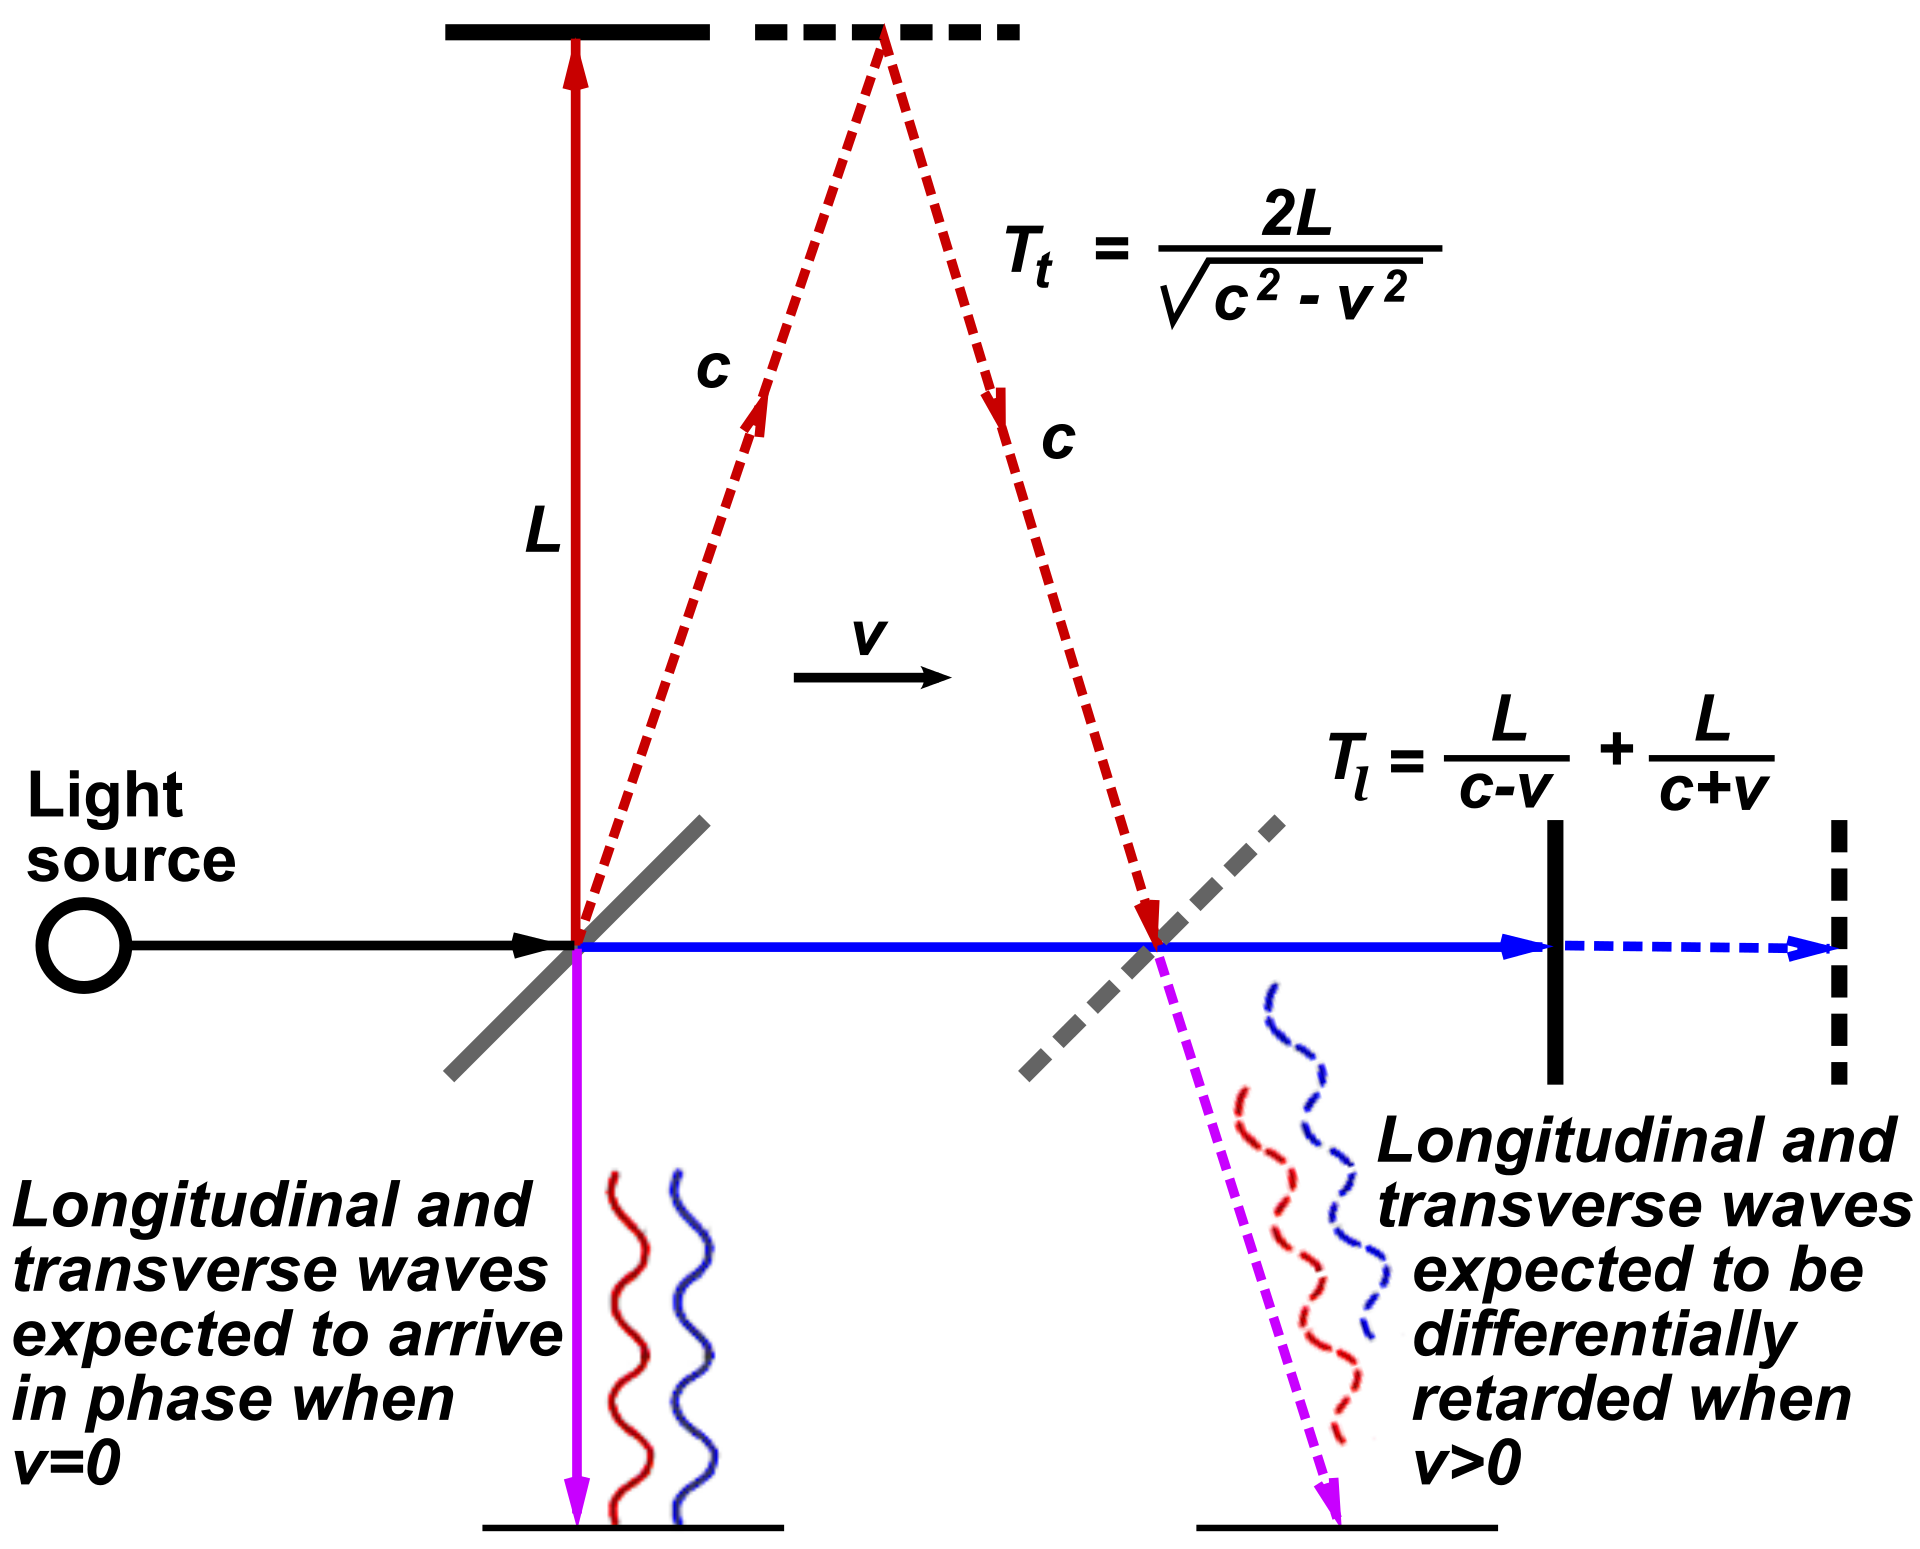
\includegraphics[width=20em,keepaspectratio]{./pictures/4.png}

          \vspace{1em}

    \item 热辐射实验-紫外灾难: 紫外波段辐射能量在当时理论下应为$\infty$,实际辐射能量为$0$
\end{itemize}

\vspace{2em}

\subsubsection{为什么要研究辐射}
\begin{itemize}
    \item 各个国家都在大炼钢铁(大炼钢时代),资本家为了提高炼钢技术请物理学家进行研究
    \item 热辐射: 任何物体都在进行热辐射(电磁波),且与\textbf{温度}(非唯一)有关
    \item 物理学家尝试测量最好炼钢温度所产生的热辐射(电磁波波谱)

          \vspace{2em}

          \begin{minipage}{0.48\textwidth}
              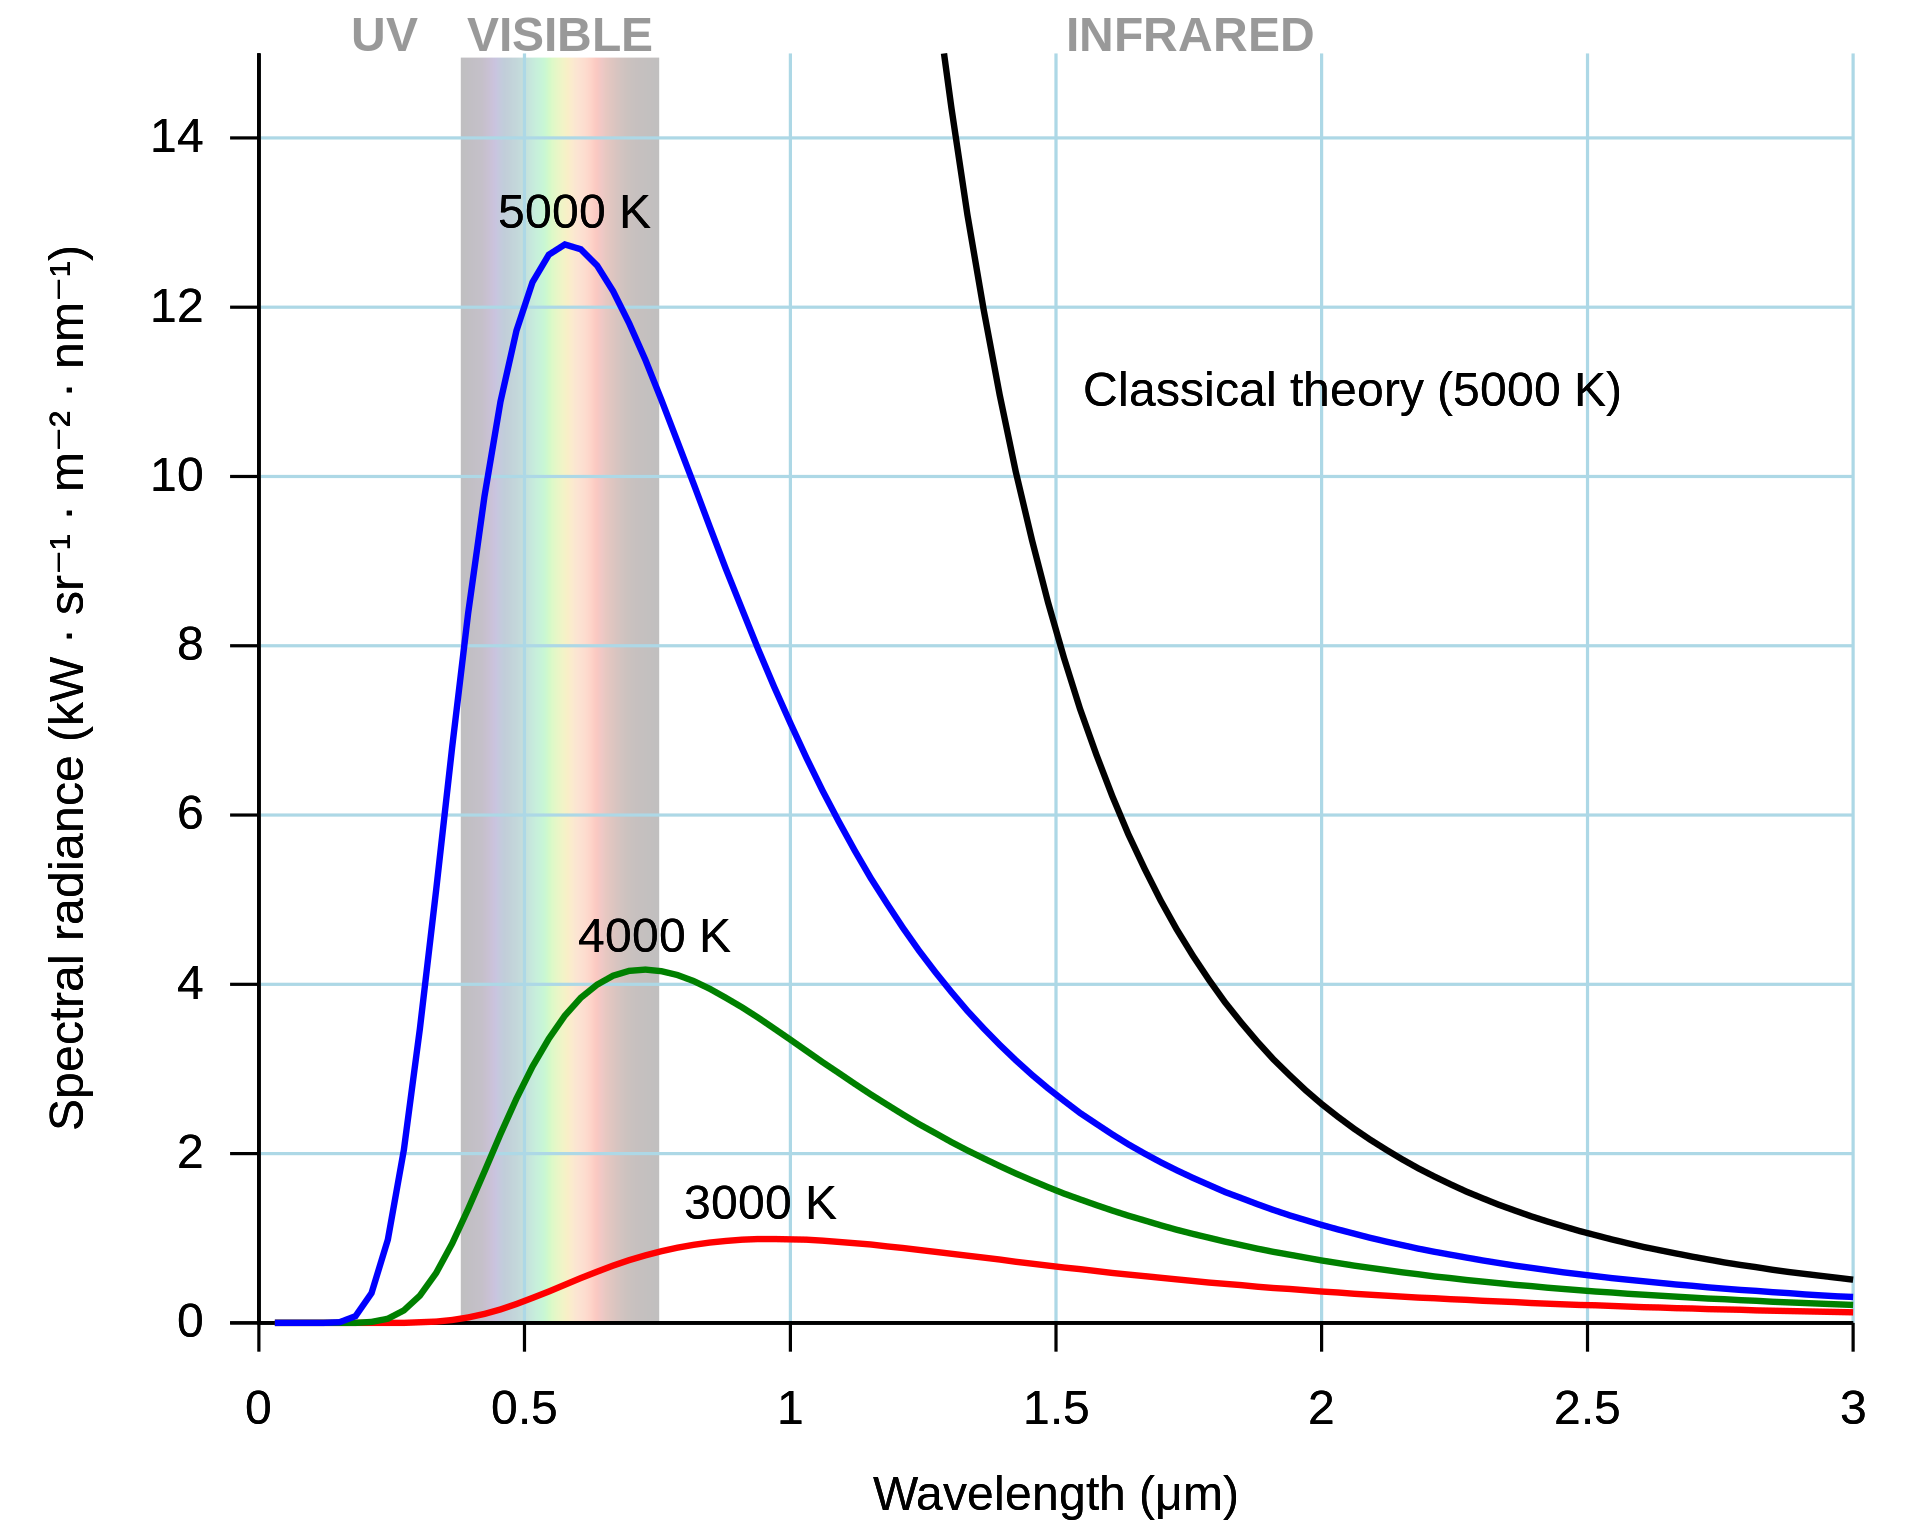
\includegraphics[width=\textwidth,keepaspectratio]{./pictures/5.png}
          \end{minipage}
          \hfill
          \begin{minipage}{0.45\textwidth}
              \vspace{-1em}
              \begin{enumerate}[label = (\arabic*)]
                  \item 在特定温度下,辐射的电磁波波段范围较广,强度不一
                  \item 随着温度的升高,辐射出的各个波段的电磁的辐射强度均升高
                  \item 随着温度升高,辐射强度最强的波长向\textbf{左}移动(频率上升)
              \end{enumerate}
              \vspace{1em}
              \begin{enumerate}[label = (\alph*)]
                  \item 维恩公式(短波接近)
                  \item 瑞利公式(长波接近) $\lra$ 紫外灾难(短波接近无穷)
              \end{enumerate}
          \end{minipage}
\end{itemize}

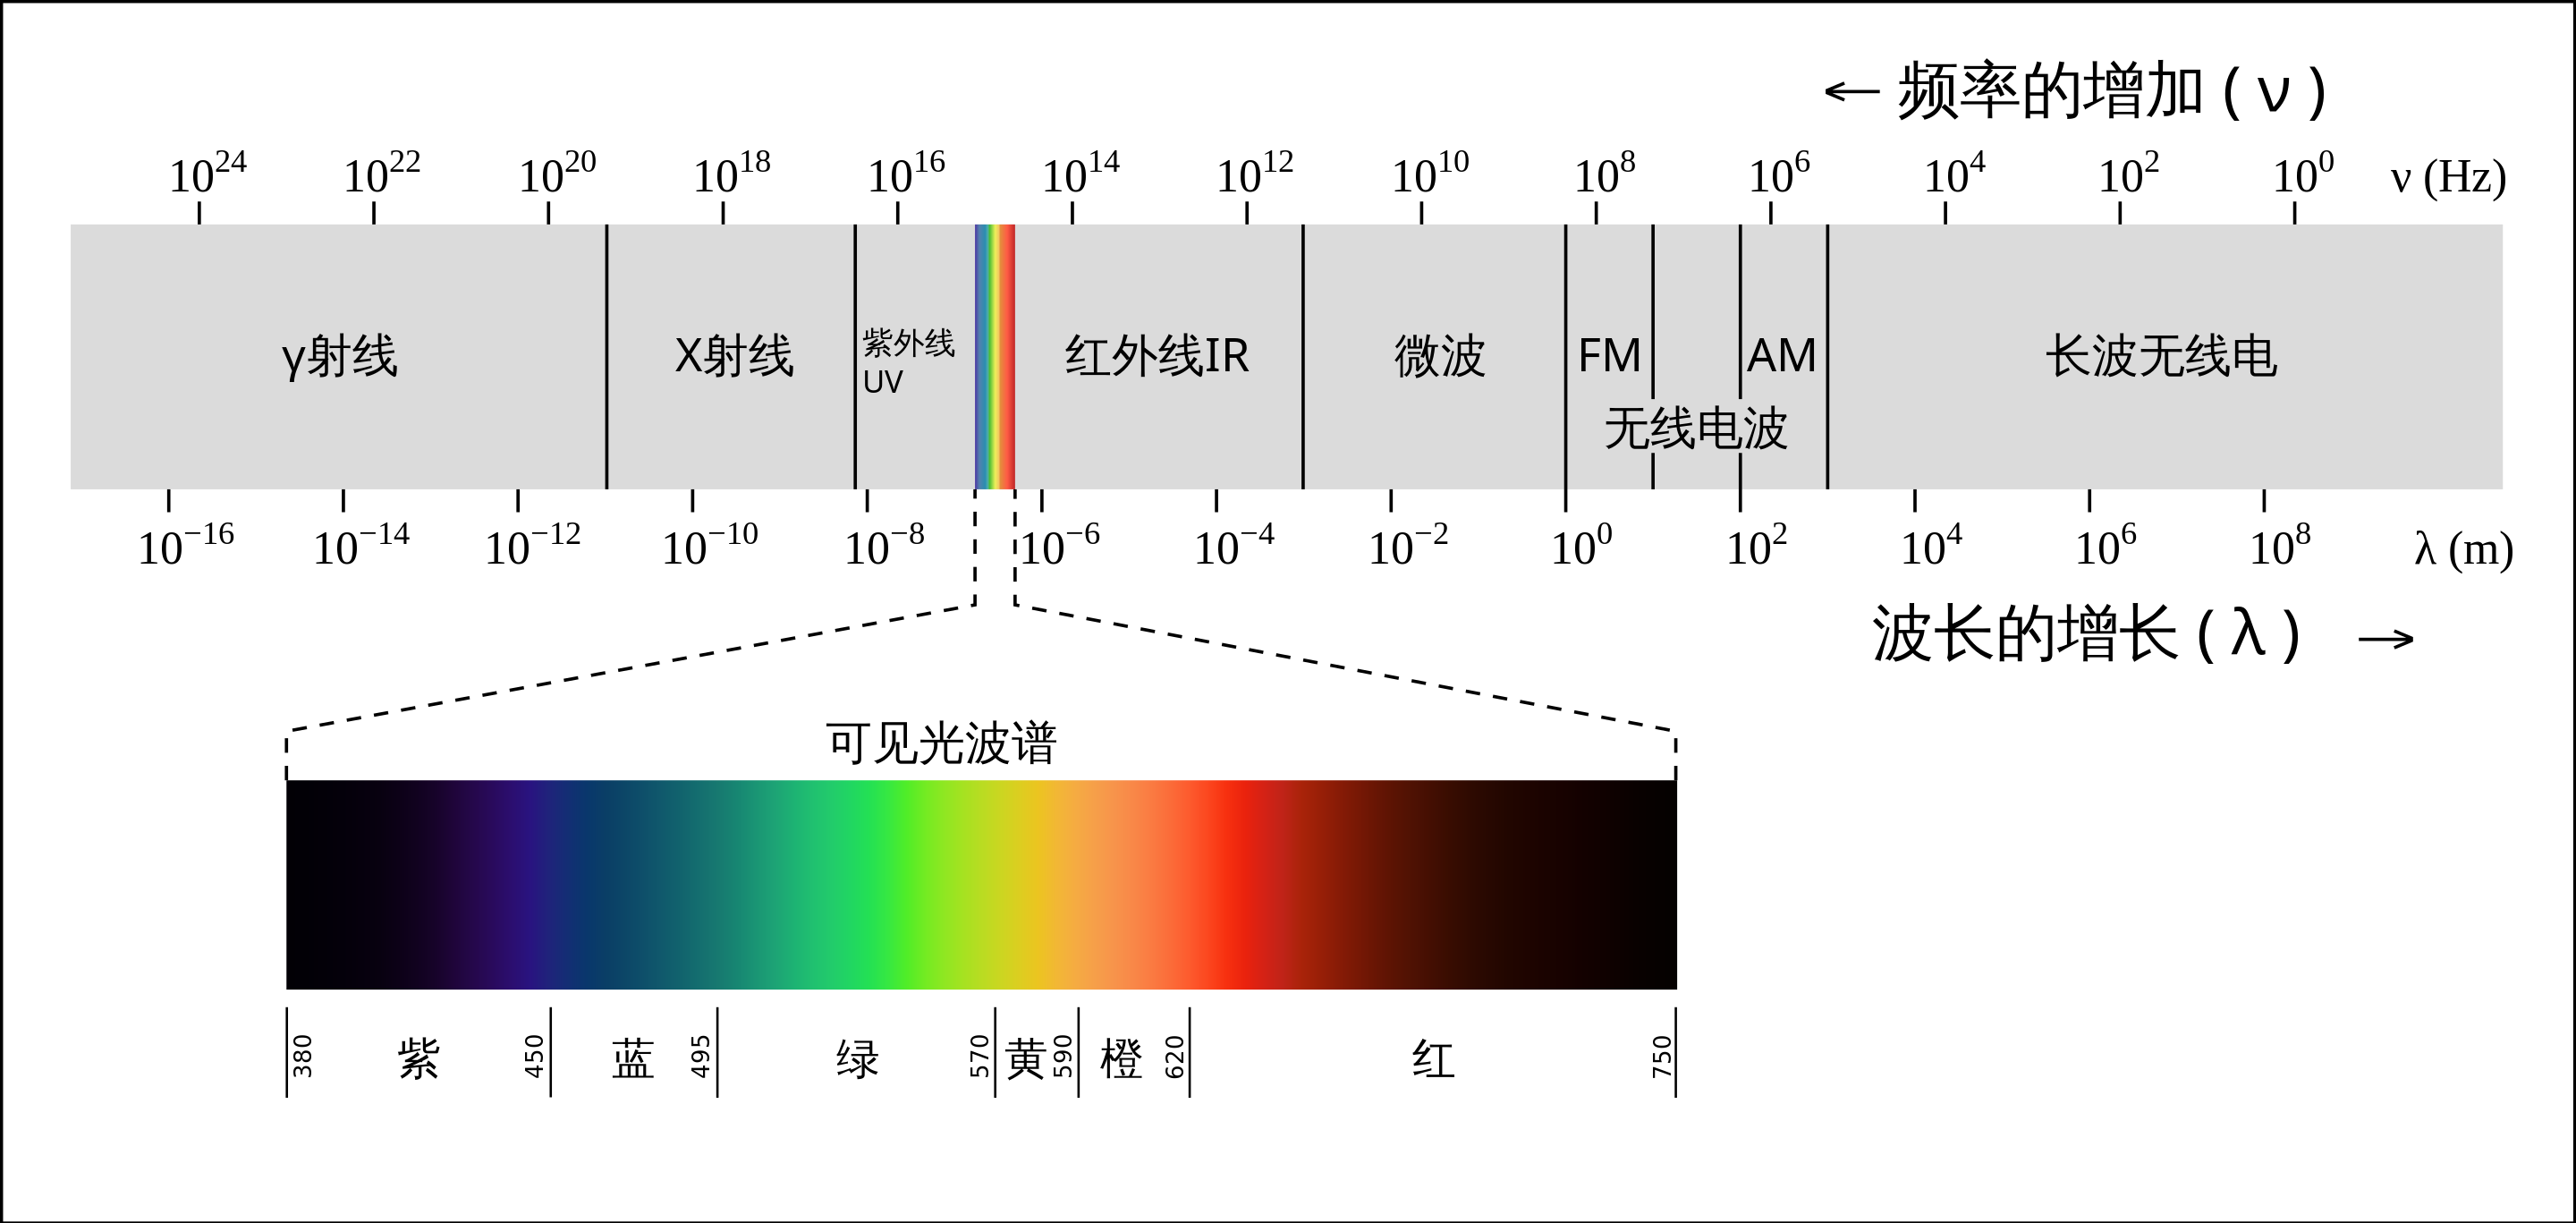
\includegraphics[width=37em,keepaspectratio]{./pictures/6.png}

\vspace{2em}

\subsubsection{黑体模型}
\begin{itemize}
    \item 理想黑体概念: 反射率与透射率为$0$,吸收率$100\%$,全靠自身发射辐射
    \item 常见近似黑体: 太阳 \, 发光灯泡 \, 钻孔箱
\end{itemize}

\vspace{2em}

\subsubsection{能量子-普朗克}

\begin{minipage}{0.4\textwidth}
    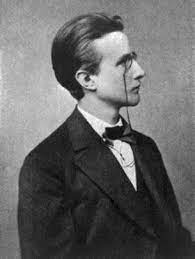
\includegraphics[width=15em,keepaspectratio]{./pictures/7.png}
\end{minipage}
\hfill
\begin{minipage}{0.4\textwidth}
    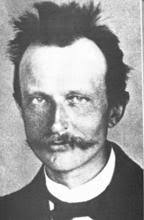
\includegraphics[width=13em,keepaspectratio]{./pictures/8.png}
\end{minipage}

\vspace{2em}

\begin{itemize}
    \item 能量子: 认为带电微粒的能量只能是某一最小能量值的整数倍,最小能量值称之为---能量子
    \item 光子: 爱因斯坦在\textbf{光电效应}现象中认为光本身由一个个不可分割的能量子组成,
          频率为$\nu$的光其能量为$h\nu$,后被称为光子
          $$
              E = h\nu    \hspace{2em}   \text{普朗克常数} \hspace{0.5em} h = 6.63 \cross 10^{-34}
          $$
\end{itemize}

\vspace{2em}

\subsubsection{光的一些描述}
\begin{itemize}
    \item 光速(传播): 真空中传播速度$3 \cross 10^{8}m/s $
    \item 频率(颜色): 单位时间内完成的周期次数$\nu$
    \item 强度(亮度): 单位时间内的光子数(粗浅定义) \, $I = nh\nu$ \, (单一光的强度改变仅改变$n$)
\end{itemize}

\vspace{2em}

\subsection{光电效应}
\subsubsection{理想模型}

\begin{minipage}{0.5\textwidth}
    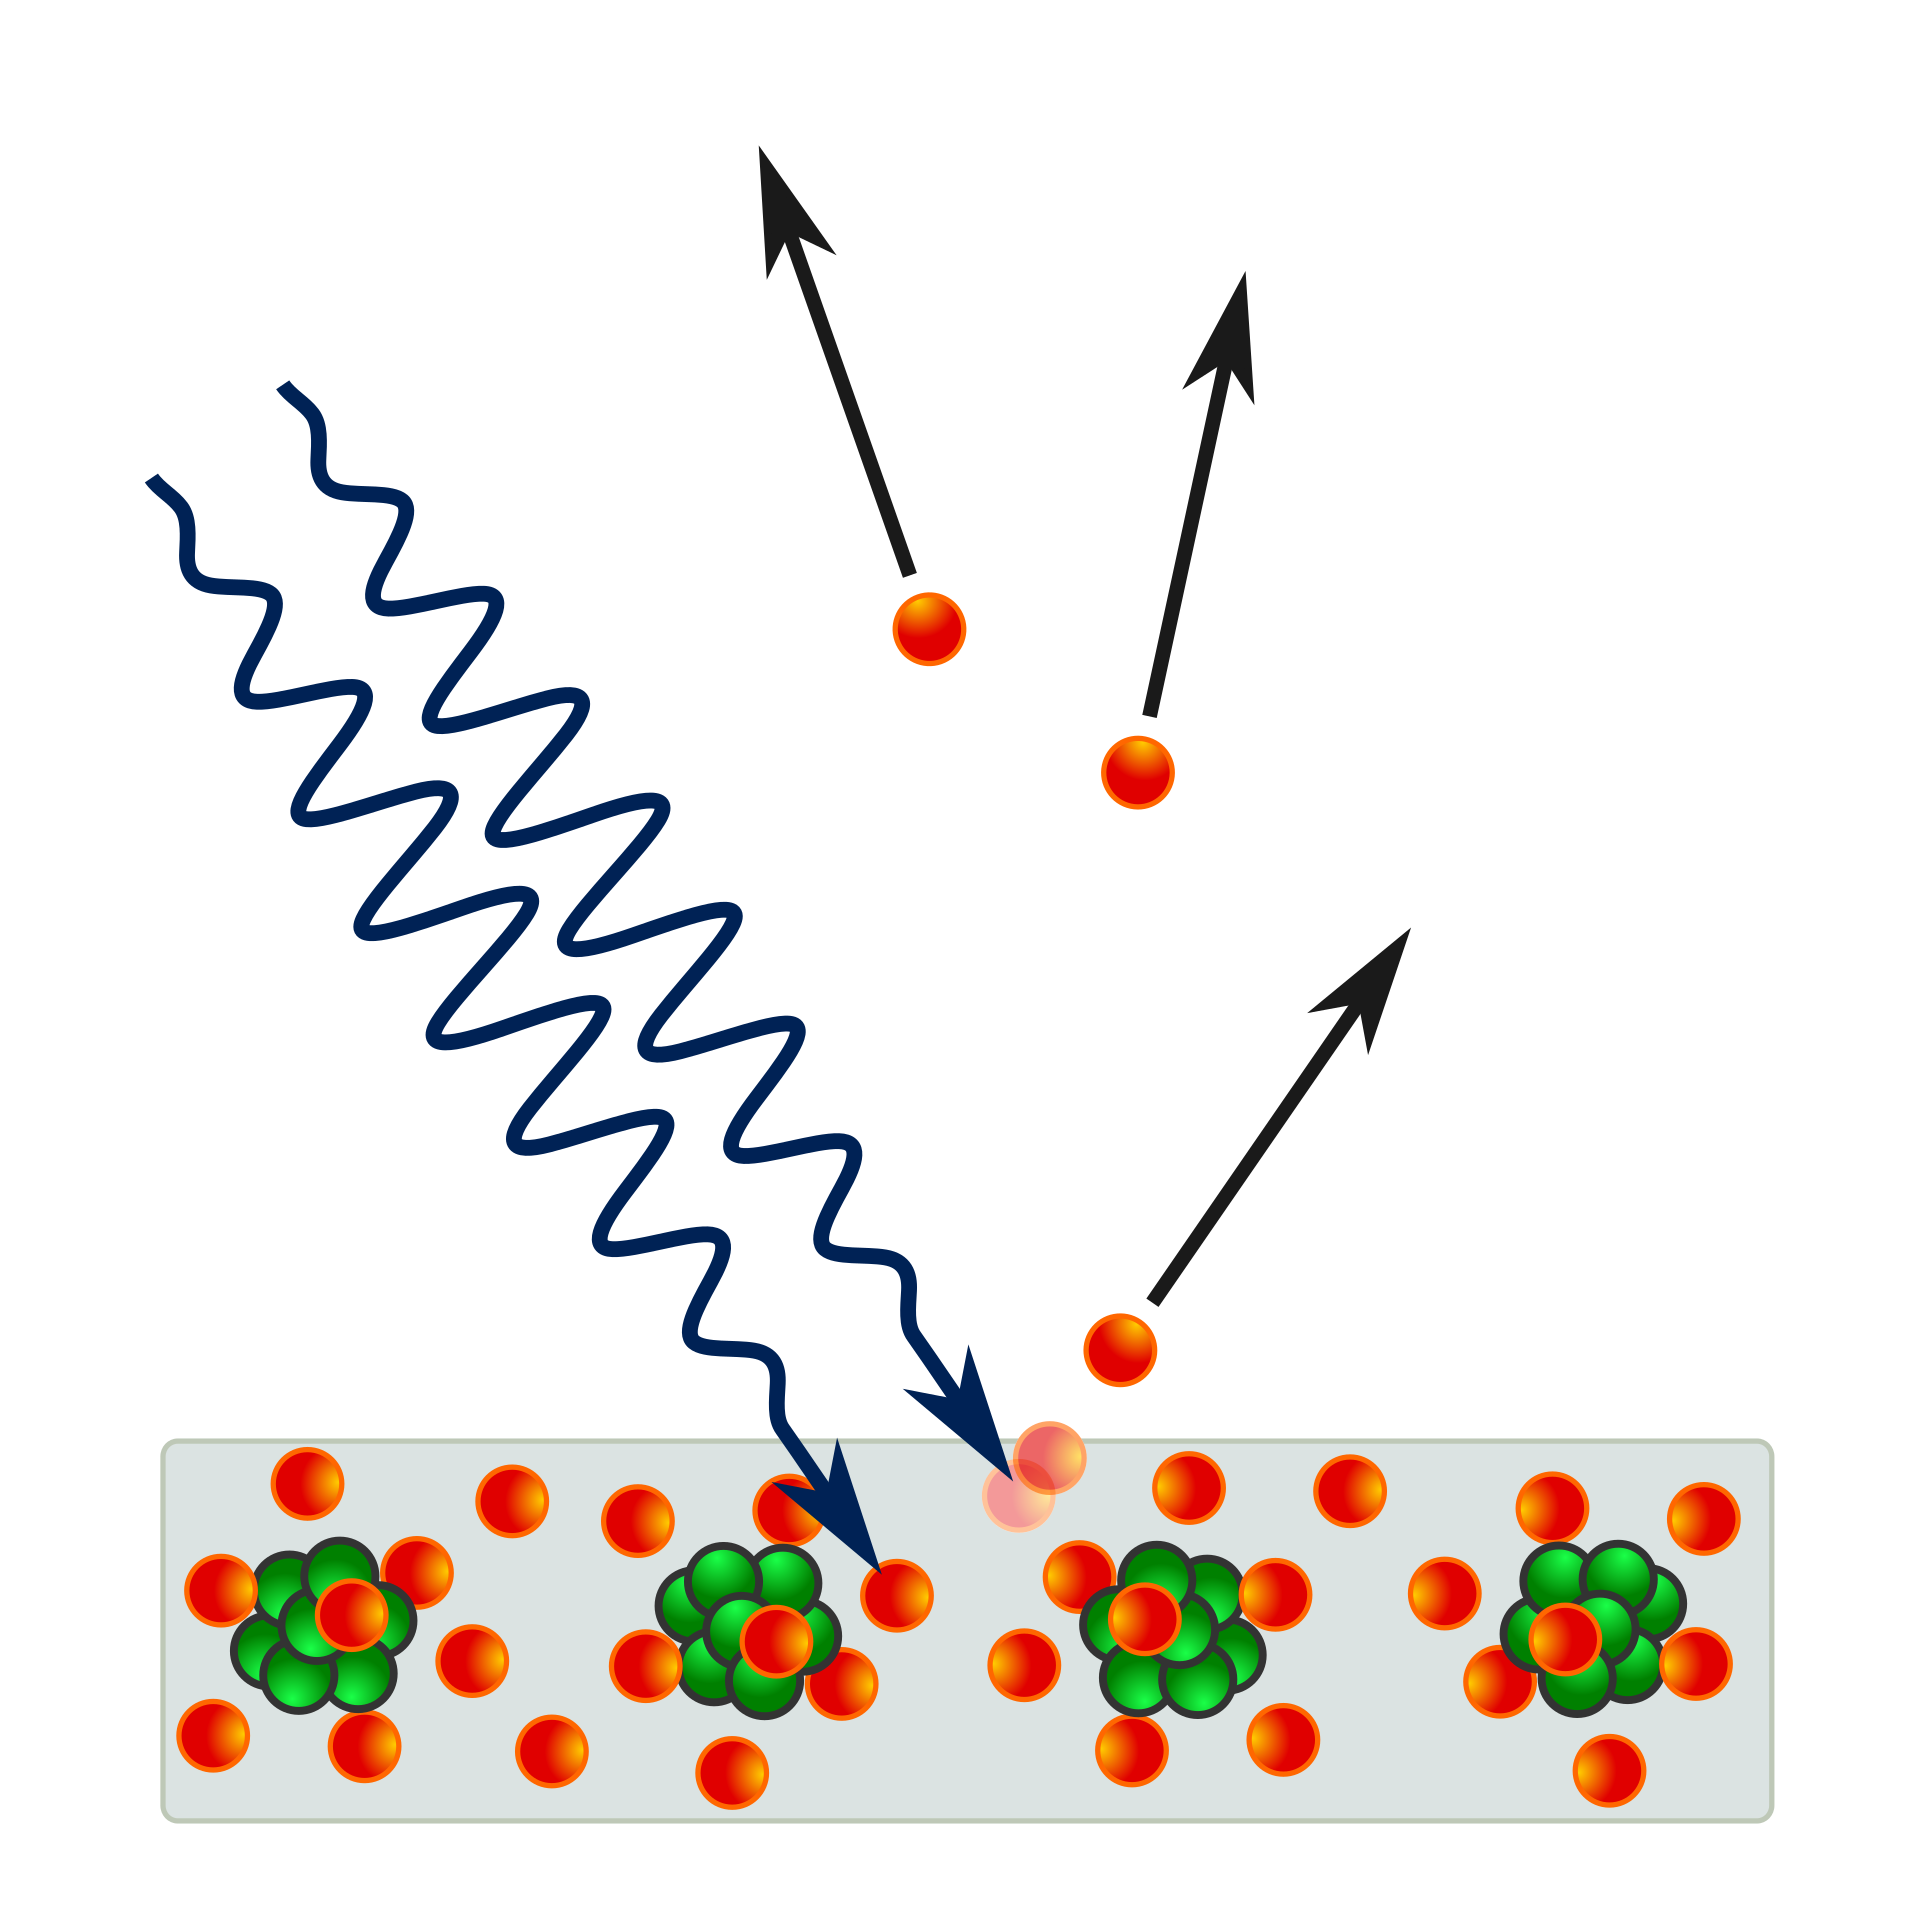
\includegraphics[width=15em,keepaspectratio]{./pictures/9.png}
\end{minipage}
\hspace{-5em}
\begin{minipage}{0.5\textwidth}
    \begin{itemize}
        \item 核外电子处于某能级上,吸收特定能量将会\textbf{跃迁}或\textbf{逃离}(电离)
        \item[]
        \item 单个光子的能量被吸收后仍有\textbf{余量},则作为电子的初动能
        \item[]
        \item 电子逃离在化学中$\llra$被氧化,这也是有些材料需要避光存储的原因
    \end{itemize}
\end{minipage}

\vspace{2em}

\subsubsection{实验雏形}
\begin{minipage}{0.5\textwidth}
    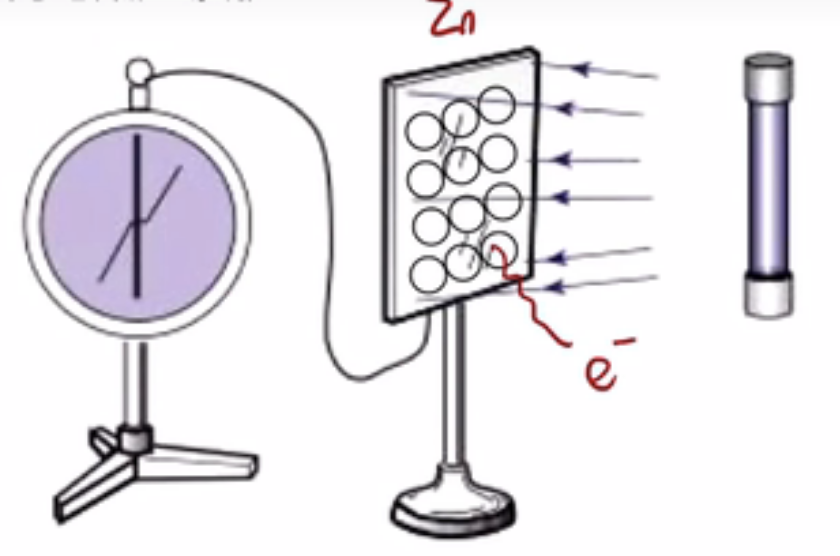
\includegraphics[width=15em,keepaspectratio]{./pictures/10.png}
\end{minipage}
\hspace{-5em}
\begin{minipage}{0.5\textwidth}
    \begin{itemize}
        \item 电子吸收能量逃离
        \item[]
        \item $Zn$板处于\textbf{正电}
        \item[]
        \item 验电器处于\textbf{正电}(工作原理:接触式起电)
    \end{itemize}
\end{minipage}

\vspace{2em}

\subsubsection{电学实验}
\begin{minipage}{0.45 \textwidth}
    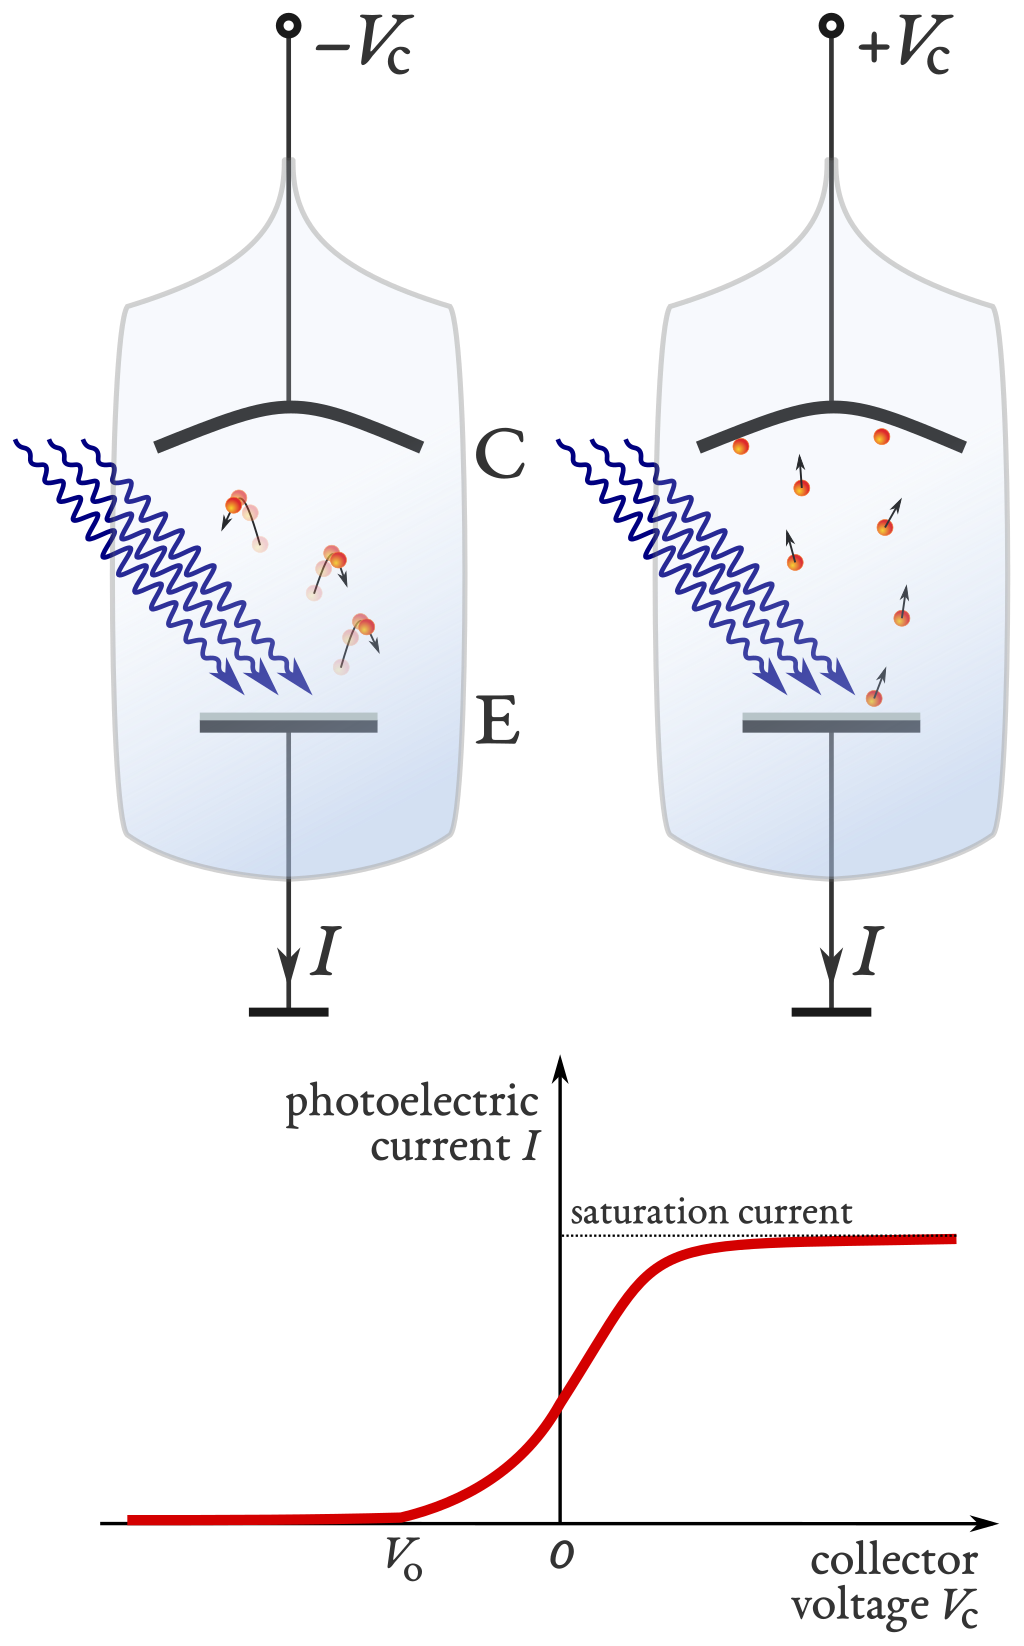
\includegraphics[width=16em,keepaspectratio]{./pictures/11.png}
\end{minipage}
\hspace{-2em}
\begin{minipage}{0.5\textwidth}
    \begin{itemize}
        \item 逸出功: 电子逃逸出金属表面所需要的最小能量 \, $W_{0}$
        \item[]
        \item 最大初动能: 一定频率光照下刚逃逸的电子所具有最大初动能 $E_{kmax} = h\nu - W_{0}$
        \item[]
        \item 饱和光电流: 所有逃逸电子均打到极板(忽略速度对电流的影响) \, $I_{s}$
              \begin{itemize}
                  \item[] 增大光频率 $\times$
                  \item[] 增加光照强度(调整$n$)$\surd$
              \end{itemize}
        \item[]
        \item 遏止电压: 恰好使得没有任何电子打到极板$V_{stop}q = E_{kmax}$ (抵消电子最大初动能)
        \item[]
        \item 截止频率(极限频率): 恰好发生光电效应时的频率$E_{kmax} \lra \nu_{0} = \frac{W_{0}}{h} $
    \end{itemize}
\end{minipage}

\vspace{2em}

\subsection{原子结构}
\subsubsection{物理学史}
\begin{enumerate}[label = \arabic*{}.]
    \item J.J汤姆孙发现了电子: 阴极射线的粒子称为电子
    \item J.J汤姆孙提出\textbf{"枣糕模型"}: 认为原子是一个球体,其中\textbf{正电荷分布均匀,电子镶嵌}其中
    \item 卢瑟福通过\, $\alpha$粒子散射实验 \, 提出\textbf{"核式结构模型"}:所有带正电部分体积很小但几乎有全部质量,电子在外运动

          \begin{figure}[h]
              \centering
              \begin{minipage}{0.48\textwidth}
                  \centering
                  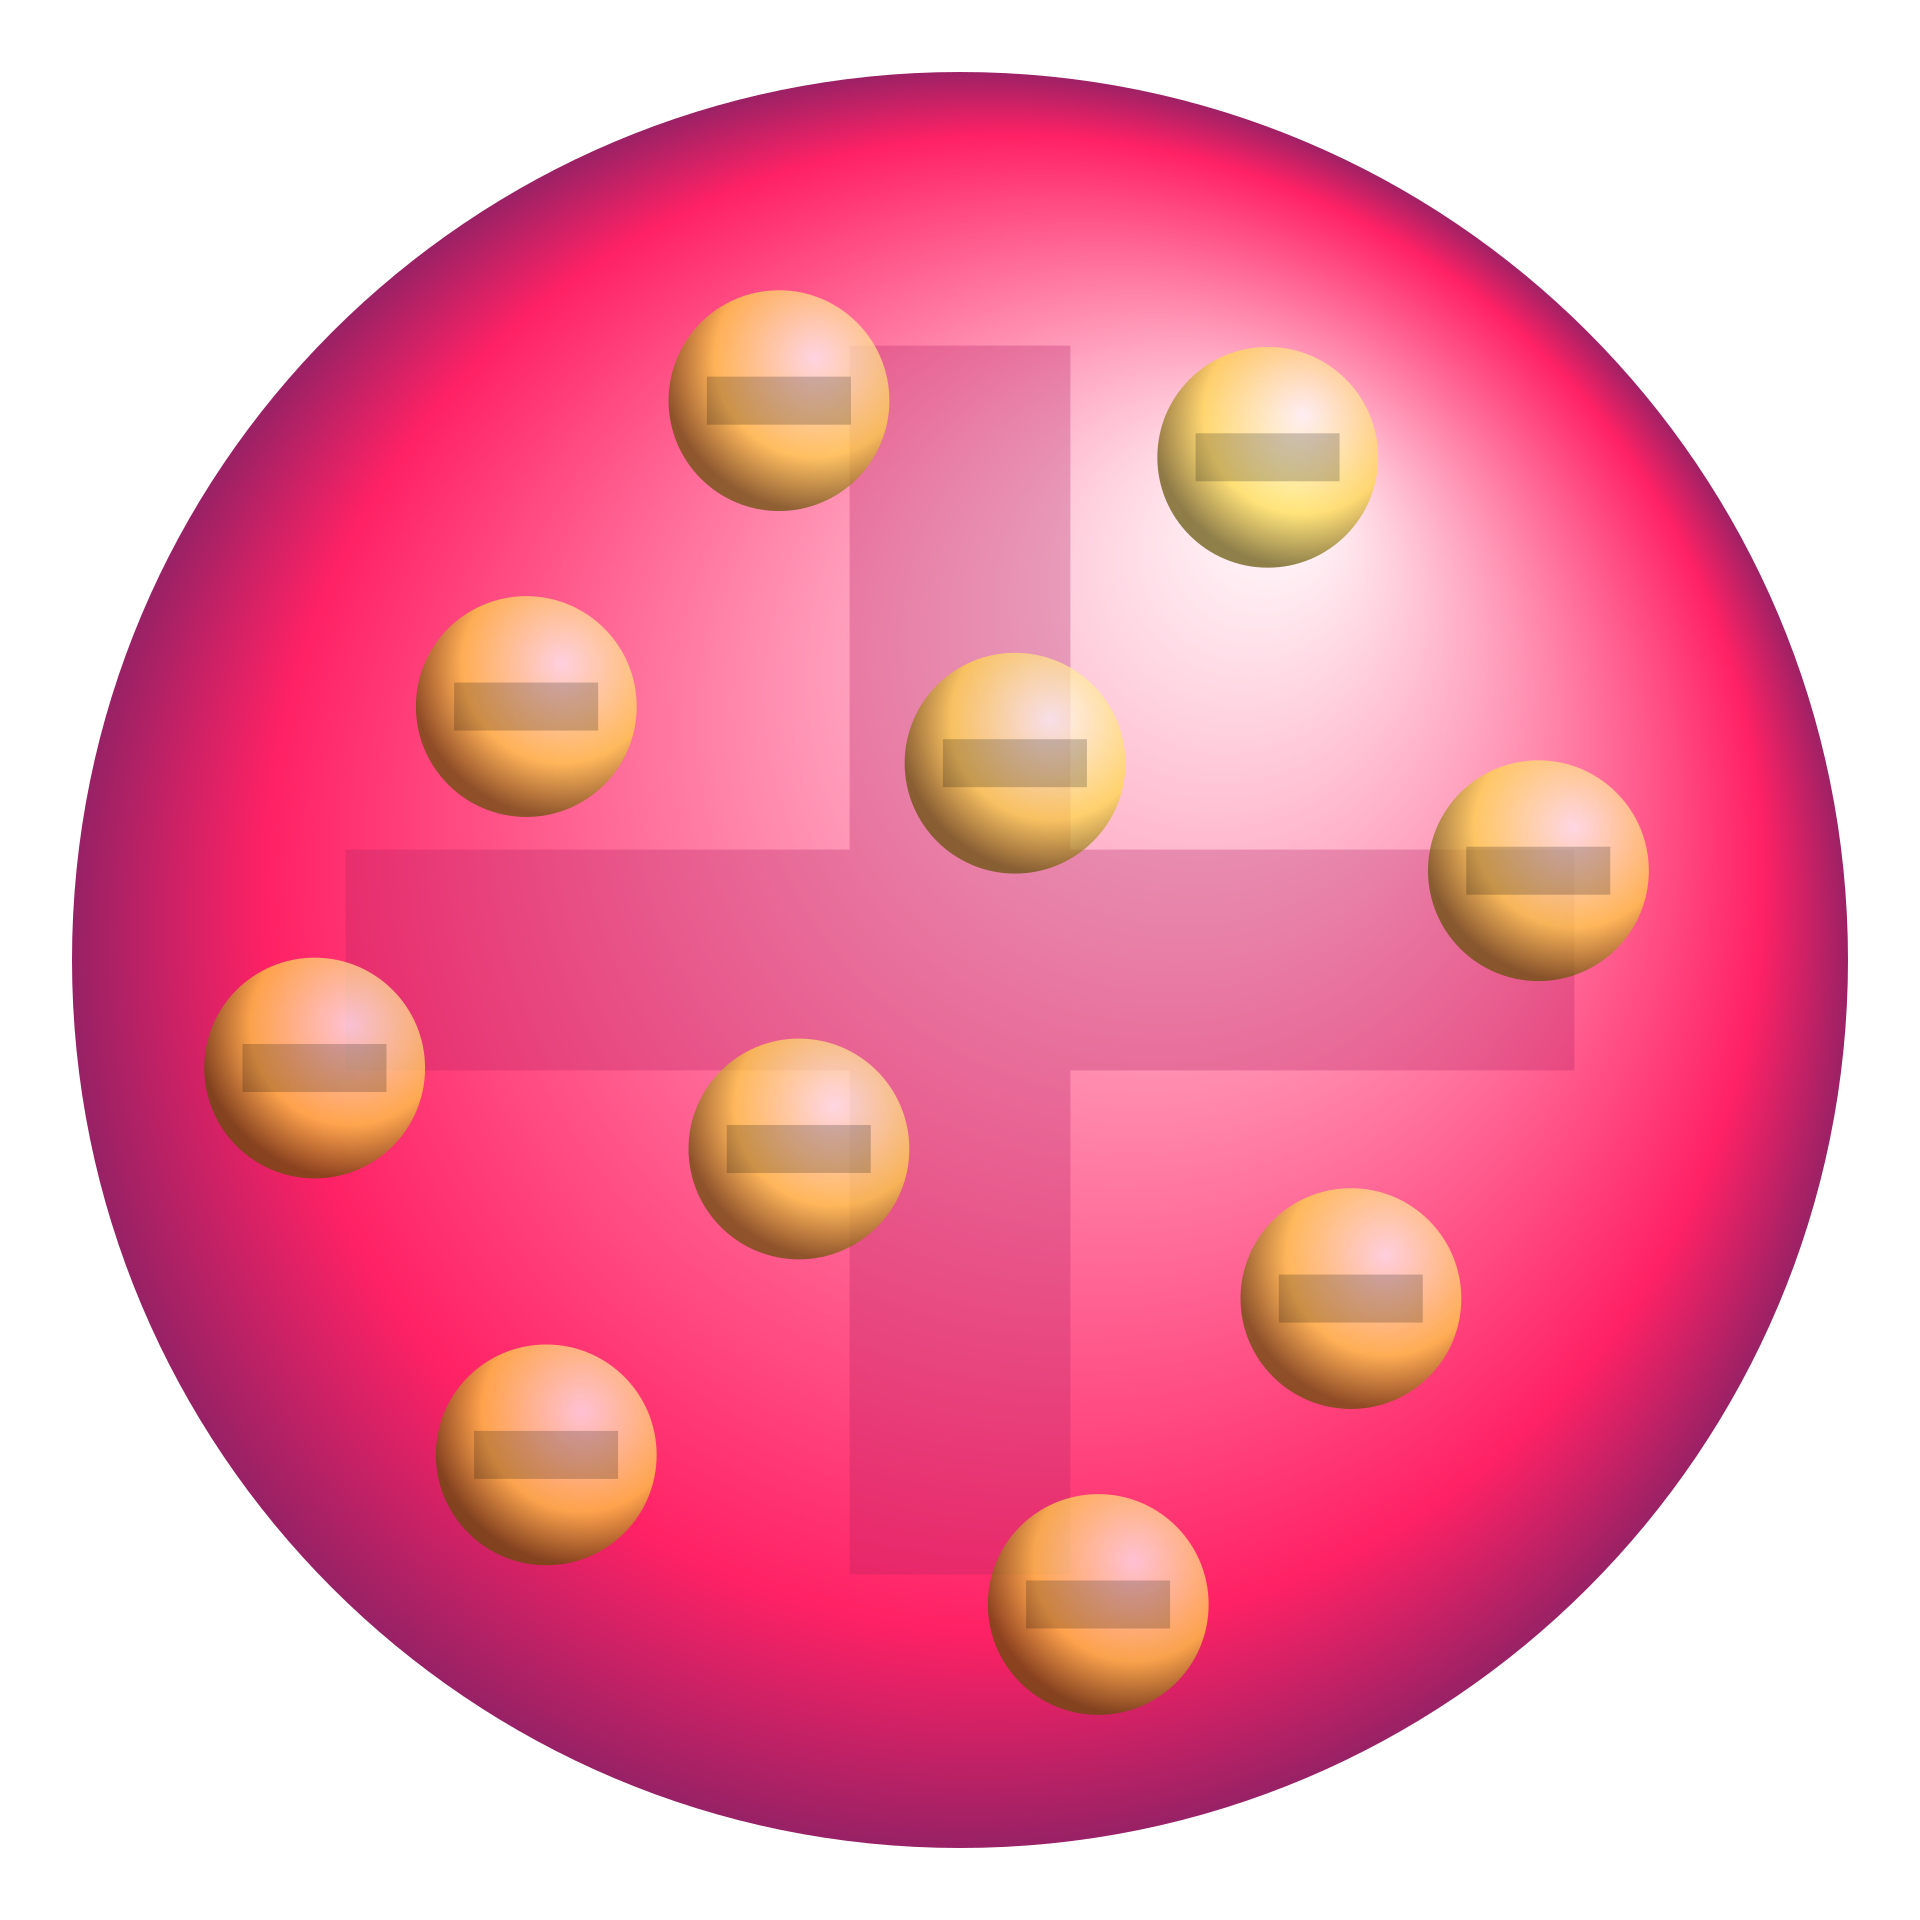
\includegraphics[width=10em]{./pictures/12.png}
                  \caption{枣糕结构}
              \end{minipage}
              \hfill
              \begin{minipage}{0.48\textwidth}
                  \centering
                  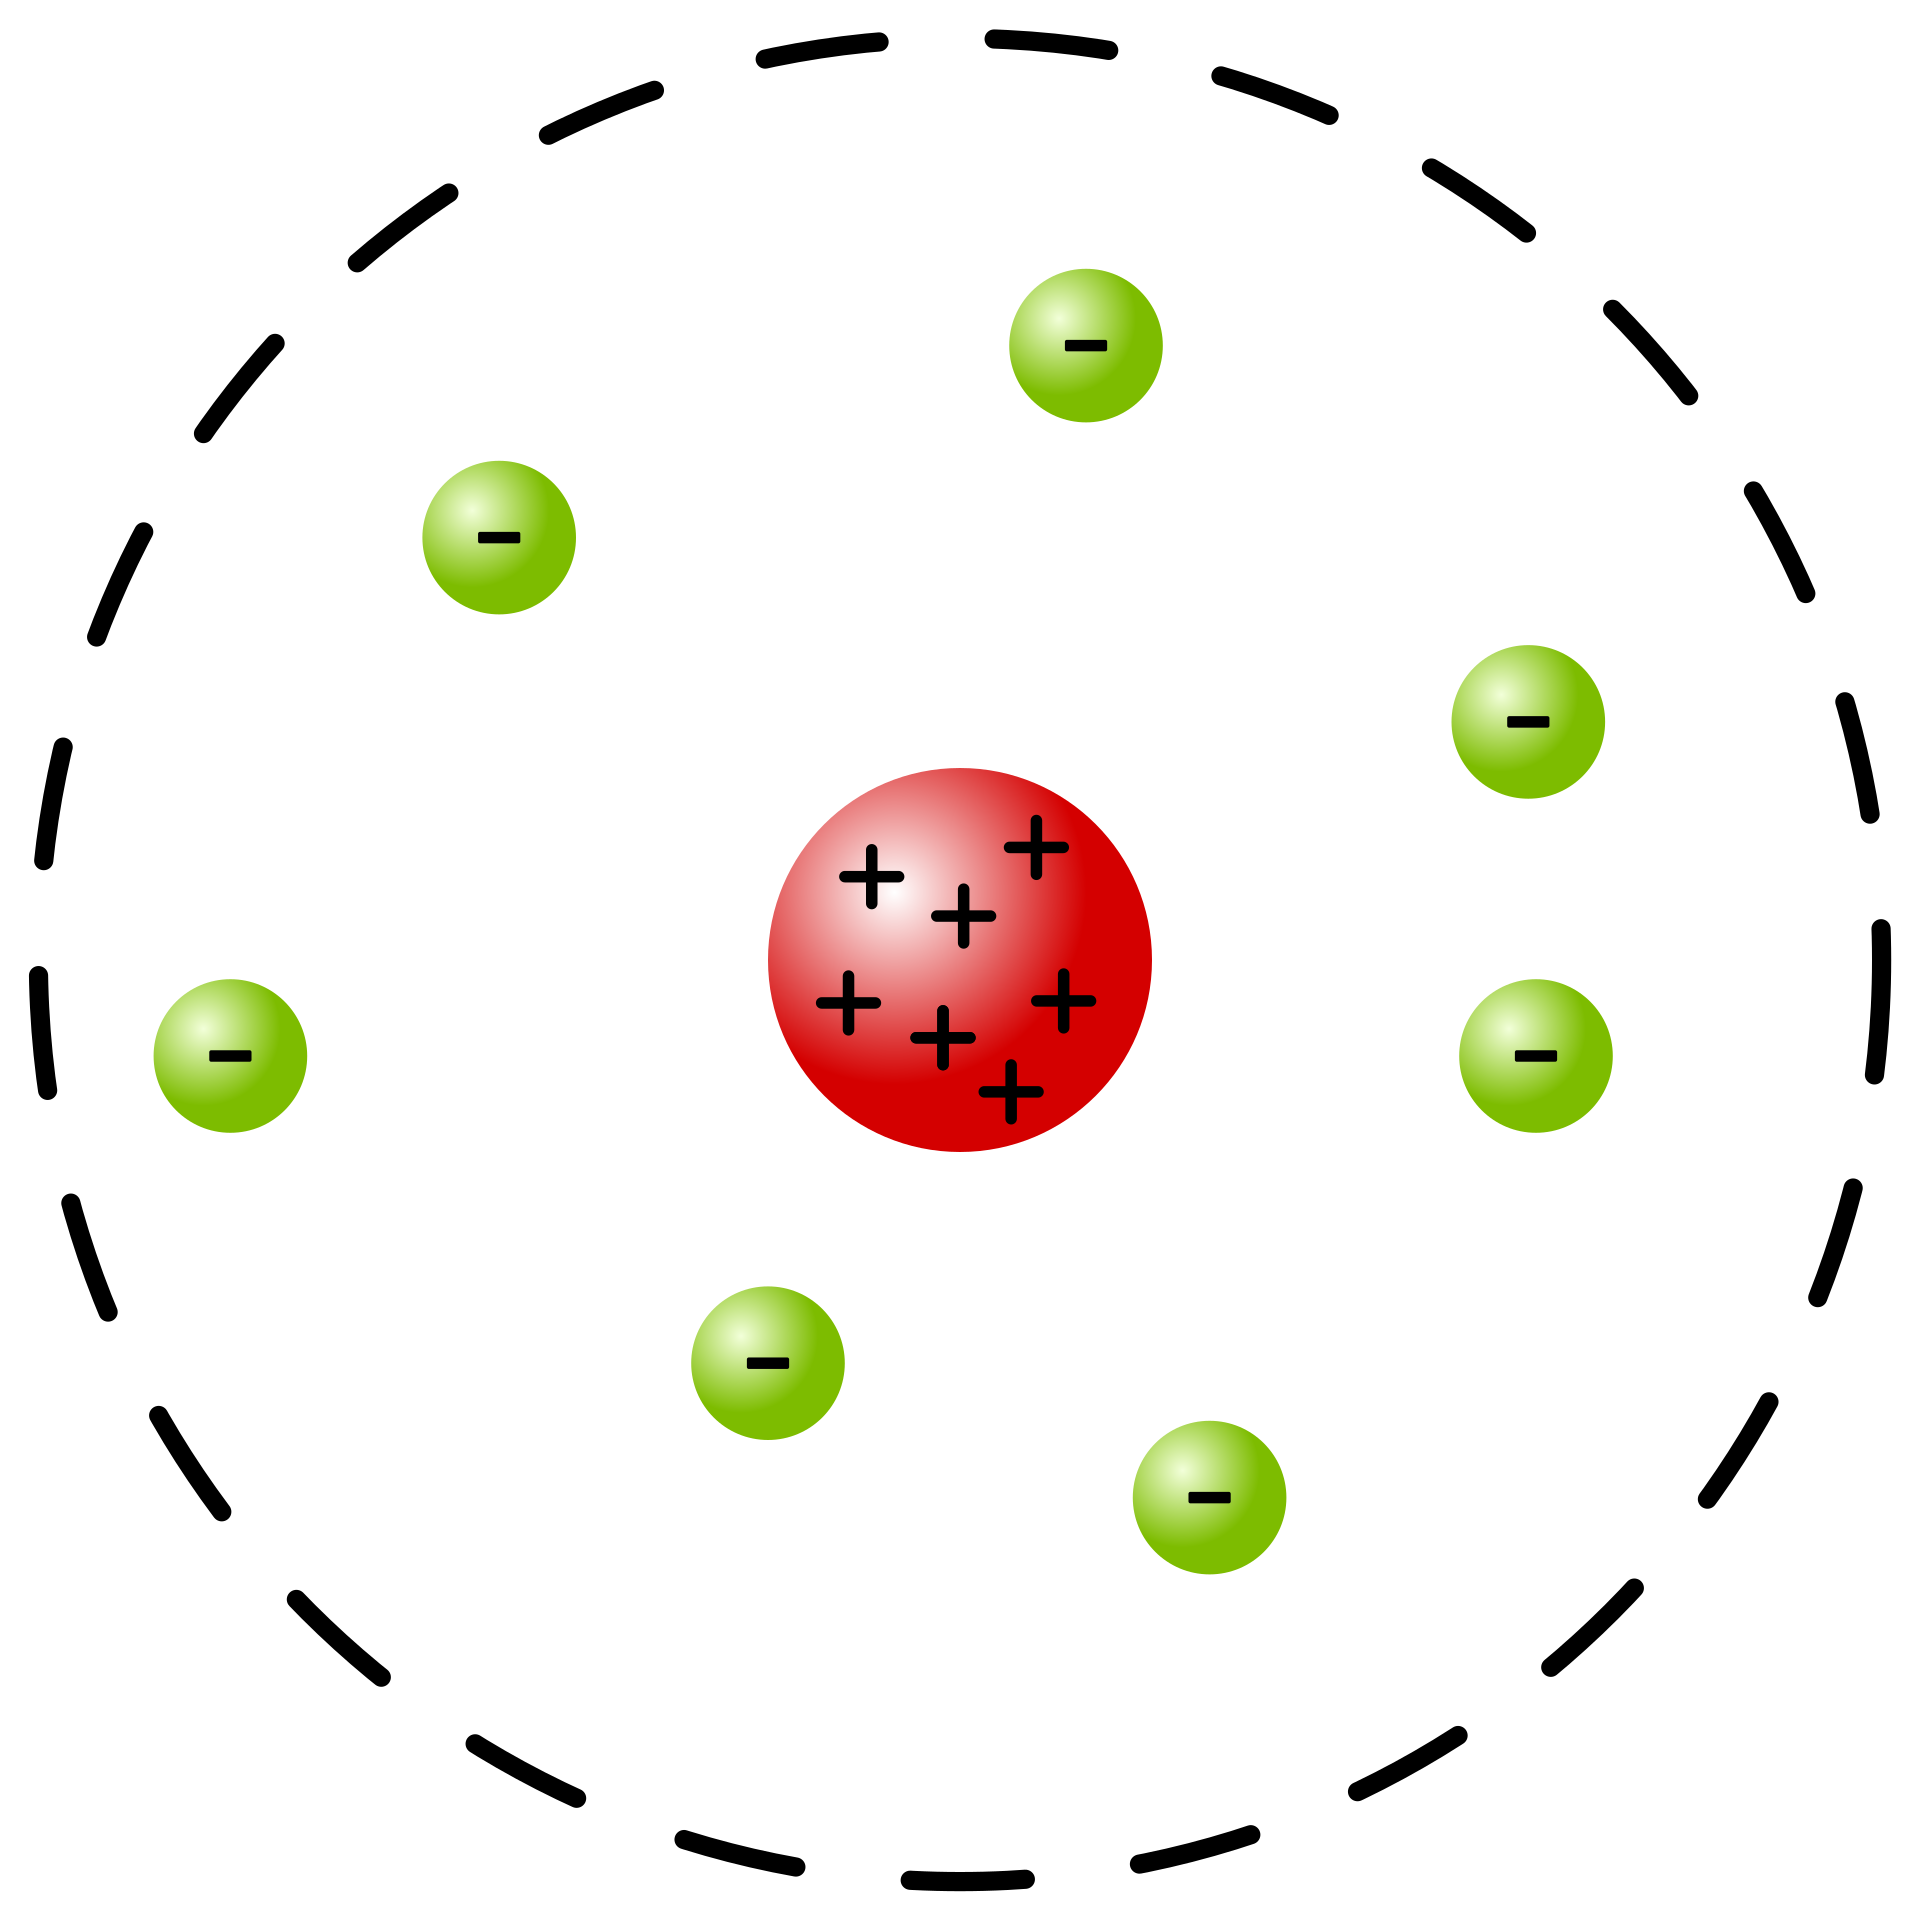
\includegraphics[width=10em]{./pictures/13.png}
                  \caption{核式结构}
              \end{minipage}
          \end{figure}
\end{enumerate}

\vspace{2em}

\subsubsection{\texorpdfstring{$\alpha$}*散射实验}
\begin{itemize}
    \item $\alpha$粒子: $He$原子核
    \item 实验原理: 使用$\alpha$粒子轰击金箔(原子间缝隙),边旋转荧光屏边接收粒子发光
    \item 实验中: 电子间的相互作用,质量,空气阻力等(极小);为何使用金箔(重,不易被碰撞影响;延展性好,可以做很薄)
    \item 实验结果
          \begin{itemize}
              \item[] 当时理论: 几乎所有粒子均可以穿过金箔
              \item[] 真实结果: 大部分穿过,少部分偏角较大,\textbf{极少部分反弹}(不符合枣糕结构模型)
              \item[] 结论: 原子内部极度空旷, 极少反弹现象是由集中的大量正电荷带来的库伦力造成
          \end{itemize}
\end{itemize}

\begin{center}
    \begin{figure}[h]
        \centering
        \begin{minipage}{0.58\textwidth}
            \centering
            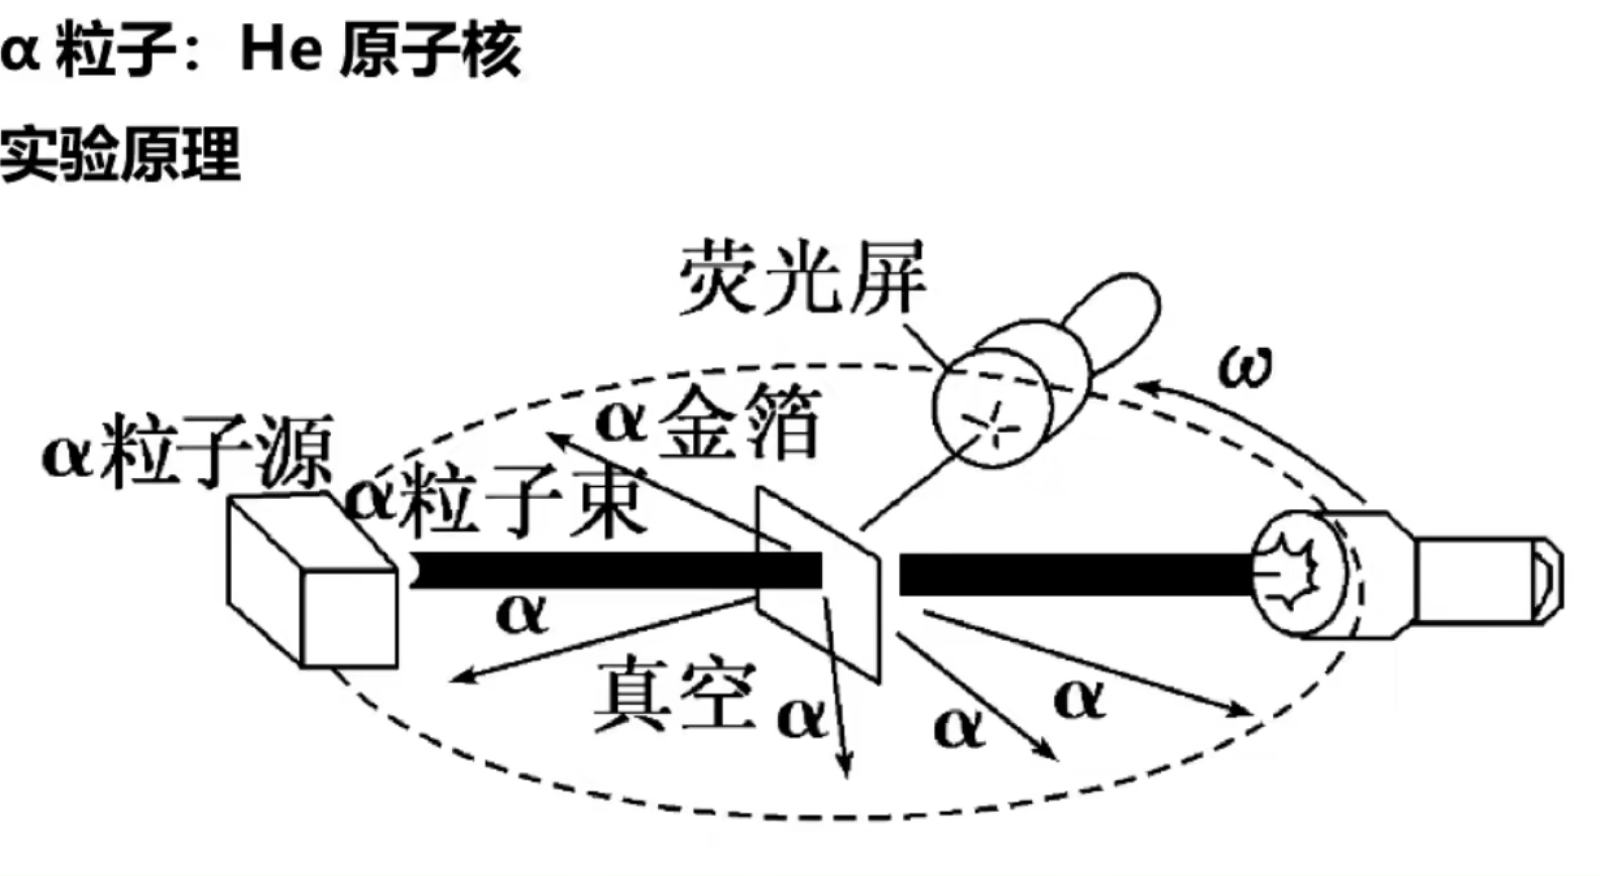
\includegraphics[width=25em]{./pictures/14.png}
        \end{minipage}
        \hfill
        \begin{minipage}{0.4\textwidth}
            \centering
            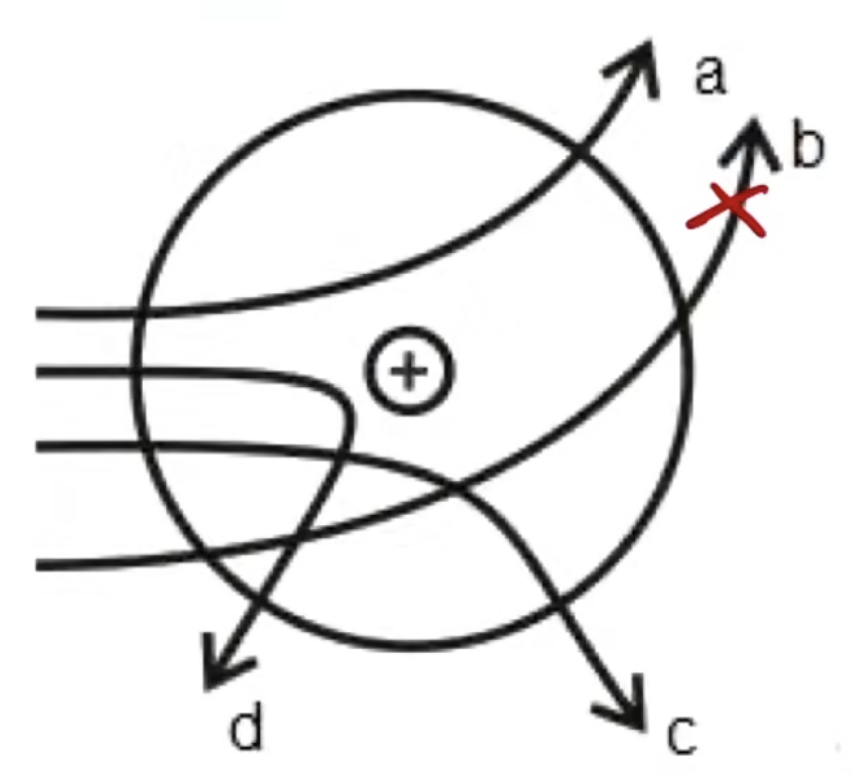
\includegraphics[width=16em]{./pictures/15.png}
        \end{minipage}
    \end{figure}
\end{center}

\vspace{2em}

\subsubsection{玻尔模型}
\begin{itemize}
    \item 经典理论的困难:
          \begin{itemize}
              \item 卢瑟福的核式结构正确指出了原子核的存在,很好的解释了$\alpha$散射实验,但是经典物理学
                    既无法解释原子的\textbf{稳定性},又无法解释原子\textbf{光谱的分立特性}.
              \item 绕核转动的电子在做周期性运动,其电磁场周期性的变化(波的传播)因而会激发电磁波,其绕核转动的能量将以电磁波的形式辐射出去.
                    所以电子绕核转动这个系统是不稳定的.然而事实是,原子是个很稳定的系统.
              \item 经典电磁理论,电子辐射的电磁波的频率就是其绕核转动频率.电子越转能量越小,那么离原子核就越来越近,转的也就越来越快,
                    这个变化应当是连续的,即应当是原子辐射各个频率的光都有(光谱应当是连续的).事实是分立的线状谱.
          \end{itemize}

          \begin{center}
              \begin{figure}[h]
                  \begin{minipage}{0.45\textwidth}
                      \centering
                      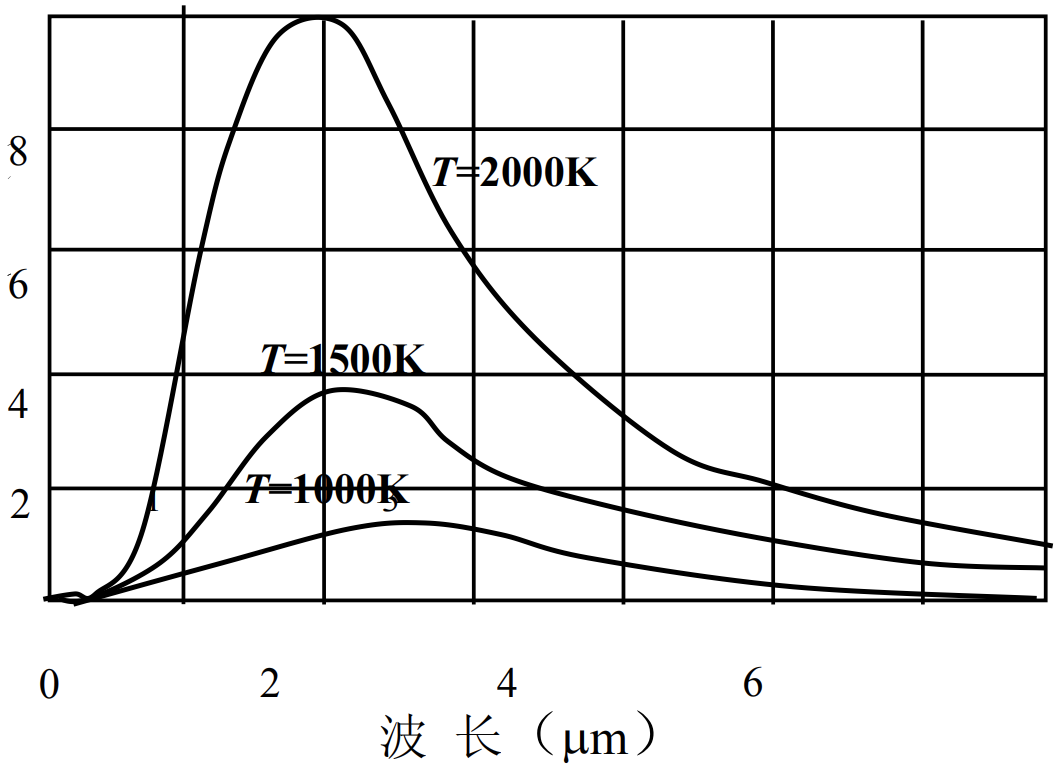
\includegraphics[width=\textwidth]{./pictures/16.png}
                      \caption*{Figure 1: 黑体辐射光谱}
                  \end{minipage}
                  \hfill
                  \begin{minipage}{0.5\textwidth}
                      \centering
                      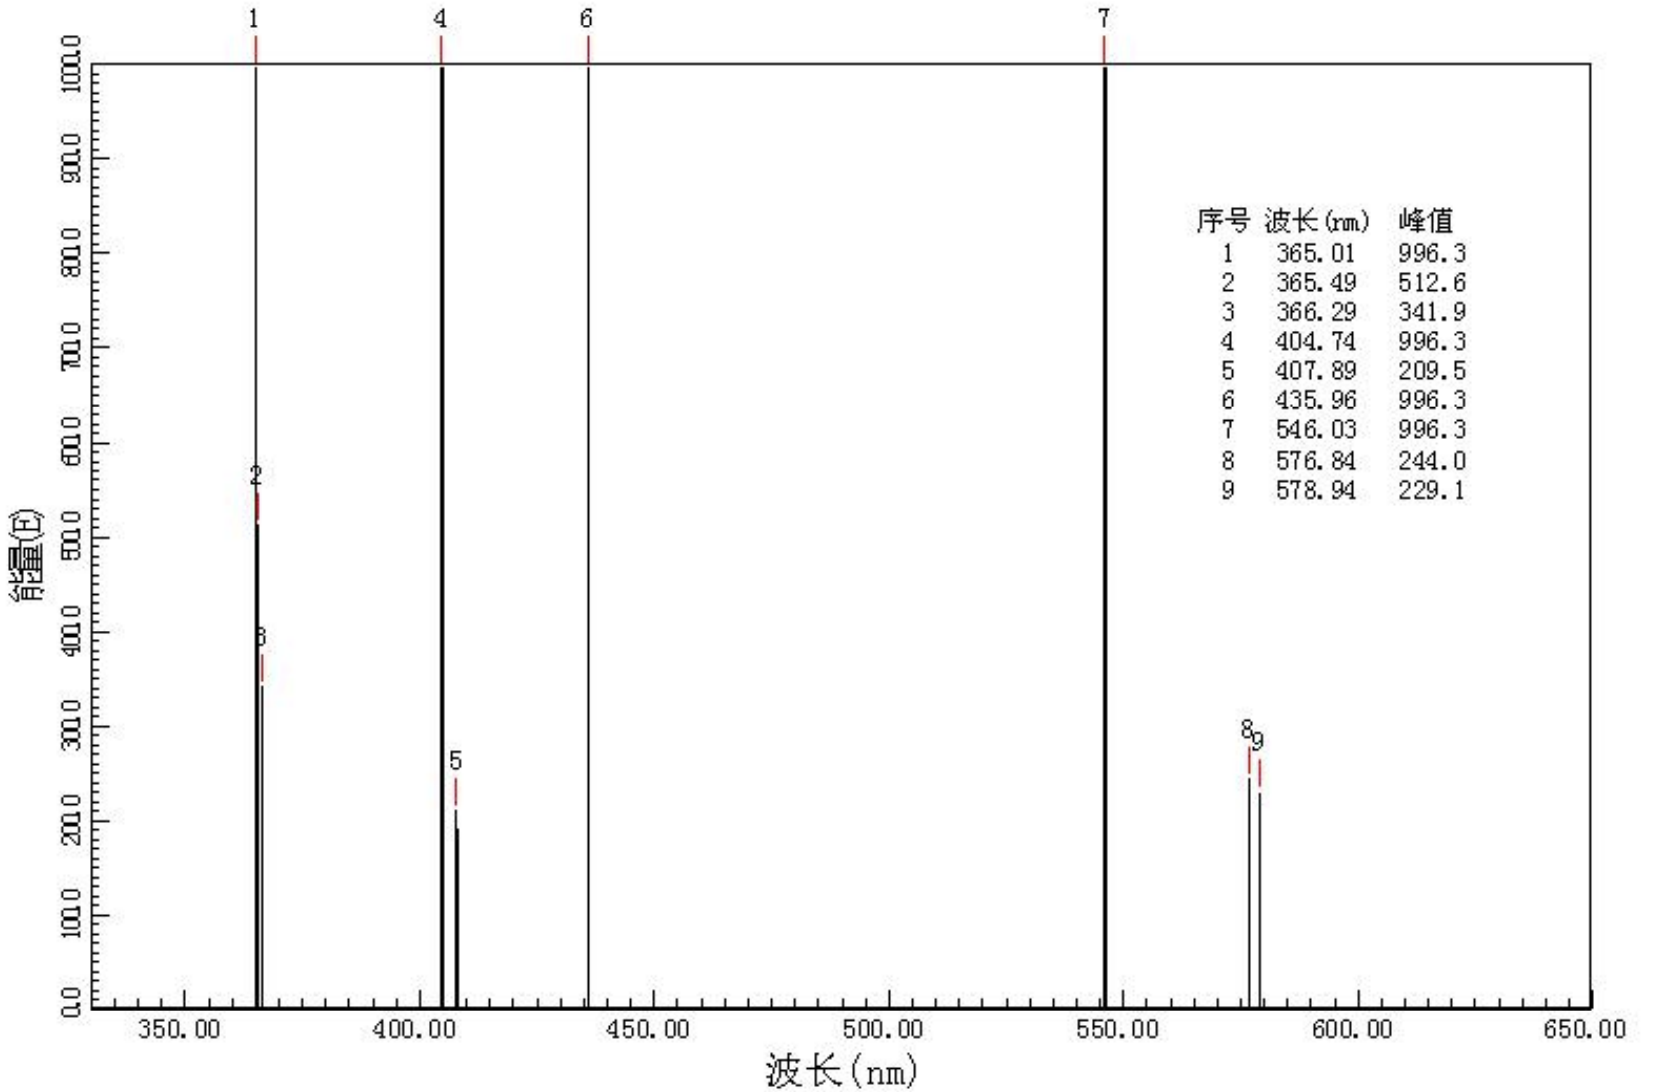
\includegraphics[width=\textwidth]{./pictures/17.png}
                      \caption*{Figure 2: 汞灯光谱}
                  \end{minipage}
              \end{figure}
          \end{center}
    \item 基本假设:
          \begin{itemize}
              \item[] 轨道量子化
              \item[]
                  \begin{minipage}{0.4\textwidth}
                      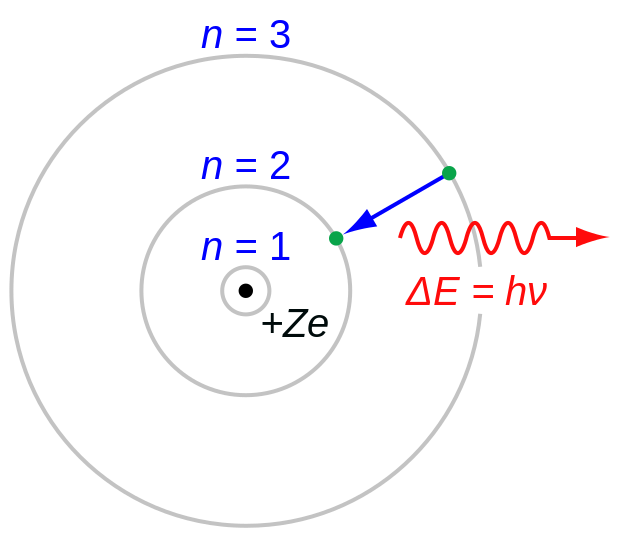
\includegraphics[width = \textwidth]{./pictures/18.png}
                  \end{minipage}
                  \hfill\hspace{-3em}
                  \begin{minipage}{0.52\textwidth}
                      \begin{itemize}
                          \item 电子\textbf{跃迁}辐射电磁波,电子在不同轨道运动$\llra$原子处于不同状态(原子跃迁)
                          \item 原子在不同的状态中具有不同的能量,因此原子的能量是\textbf{量子化},这些量子化的能量叫做\textbf{能级}
                          \item 原子中具有确定能量的稳定状态称为\textbf{定态}
                          \item 能量最低的态叫做\text{基态}$ n = 1 $;\textbf{激发态}$ n > 1 $(第一激发态$ n = 2 $)
                          \item[]
                              $\text{状态标识} \quad n = 1, \, 2, \, 3 \cdots$

                              $\text{能量标识} \quad E_{1}, \, E_{2}, \, E_{3}, \cdots$
                      \end{itemize}
                  \end{minipage}

                  \vspace{3em}

              \item[] 氢原子能级(以能级差示意跃迁难度)
              \item[]
                  \begin{minipage}{0.4\textwidth}
                      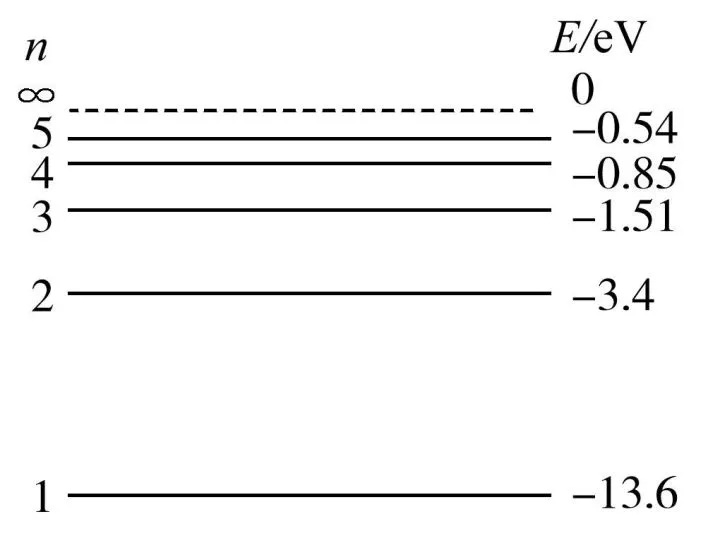
\includegraphics[width = \textwidth]{./pictures/19.png}
                  \end{minipage}
                  \hfill\hspace{-3em}
                  \begin{minipage}{0.52\textwidth}
                      \begin{itemize}
                          \vspace*{-2em}
                          \item $E_{1}=-13.6eV \,\, E_{2} = -3.6eV \,\, E_{3} = -1.51eV $
                                $$E_{n} =  \dfrac{E_{1}}{n^{2}}$$
                          \item 电子吸收能量的方式:
                                \begin{itemize}
                                    \item[] \textbf{恰好}拥有某两能级差的光子(区别于光电效应中对光能量吸收的要求)
                                    \item[] \text{大于}某两能级差的实物粒子撞击
                                \end{itemize}
                          \item 电离: 电子吸收能量完全逃离(最远处能级为$0$)原子核的束缚
                      \end{itemize}
                  \end{minipage}
          \end{itemize}
    \item 电子跃迁(从高$\ra$低)
          \begin{itemize}
              \item 处于激发态的电子是不稳定的,将会\textbf{自发}从高能级向低能级跃迁
              \item 向低能级跃迁过程中会发射\textbf{特定频率}的电磁波(光)
              \item 有多种向低能级跃迁的方法时,跃迁结果不定,直至跃迁到基态
              \item 大量处于同一激发态的电子,所能发射电磁波的频率的种类最多$C_{n}^{2} = \frac{n(n-1)}{2}$
          \end{itemize}
\end{itemize}

\vspace{2em}

\subsection{天然放射性现象}
\begin{itemize}
    \item 定义: 放射性元素\textbf{原子核内部自发}放出射线的现象
    \item 三种射线:
          \begin{itemize}
              \item[] $\alpha$射线: $^{2}_{4}He$原子核 \, 速度$0.1c$
              \item[] $\beta$射线: $^{-1}_{0}e$ \, 速度$0.99c$
              \item[] $\gamma$射线: $^{0}_{0}n$电磁波 \, 速度$c$
              \item[] 电离能力: 使得被射线辐射的物质发生电离的能力 $\alpha > \beta > \gamma$

                  \vspace{-1em}
                  \begin{adjustbox}{minipage=0.91\linewidth, bgcolor=gray!20, padding=1em}
                      \small
                      距离足够近,放射性同位素释放出的$\alpha$粒子就足以穿透皮肤从而杀死皮下的重要组织的细胞.
                      相比$\gamma$射线和$x$光对细胞造成毁伤的能力,$\alpha$射线对细胞所造成的损坏程度超过其二十倍以上
                  \end{adjustbox}
                  \vspace{-1em}

              \item[] 穿透能力: 穿透物质能力 $\gamma > \beta > \alpha$ \, (甚至不能穿透一张纸)
              \item[] 磁场半径: $ r = \dfrac{mv}{qB} \quad q_{\alpha} = 2 q_{\beta}
                      \quad m_{\alpha} \gg m_{\beta} \lra r_{\alpha} > r_{\beta} $
              \item[] 电场偏转: $ a = \dfrac{Eq}{m} \quad q_{\alpha} = 2 q_{\beta}
                      \quad m_{\alpha} \gg m_{\beta} \lra a_{\alpha} < a_{\beta} $

                  \vspace{-1em}
                  \begin{adjustbox}{minipage=0.4\linewidth, bgcolor=gray!20, padding=1em}
                      \small
                      $\beta$粒子相比$\alpha$粒子在电磁场中更易发生偏转
                  \end{adjustbox}
                  \vspace{-1em}
          \end{itemize}
\end{itemize}

\vspace{2em}

\subsection{放射性元素的衰变}
\begin{enumerate}
    \item 原子核的表示: $_{Z}^{A}X$ \quad ($A$表质量数,$Z$为原子核的电荷数 \, eg. $_{4}^{2}He$)

          \vspace{-1em}
          \begin{adjustbox}{minipage=0.32\linewidth, bgcolor=gray!20, padding=1em}
              \small
              同位素: \, 质子数一样,质量数不一样
          \end{adjustbox}
          \vspace{-1em}

          \vspace*{2em}

    \item 衰变形式:
          \begin{itemize}
              \item $\alpha$衰变: 放射性元素原子核放出$\alpha$粒子
                    $$
                        \nuc{238}{92}{U} \xlongrightarrow{\quad\quad} \nuc{234}{90}{Th}  + \nuc{4}{2}{He}
                    $$
              \item $\beta$衰变: 放射性元素原子核放出$\beta$粒子(非核外电子,中子$\ra$电子$+$质子)

                    \hspace{4em}$\beta$衰变不改变质量数(未知衰变的计算方法)
                    $$
                        \nuc{234}{90}{Th} \xlongrightarrow{\quad\quad}  \nuc{234}{91}{Pa}+ \nuc{0}{-1}{e}
                    $$
              \item $\gamma$衰变: $\alpha$衰变,$\beta$衰变过程中会伴随着$\gamma$射线
              \item 衰变的轨迹分析: eg.进行$\alpha$衰变并处在$X$磁场下
                    \begin{align*}
                         & r = \frac{mv}{qb} \quad \text{由动量守恒}  \quad \abs{m_{\alpha}v_{\alpha}} = \abs{m_{\text{核}}v_{\text{核}}} \\
                         & q_{\text{核}} > q_{\alpha} \hspace*{7em} r_{\text{核}} < r_{\alpha}
                    \end{align*}
              \item[] \hspace*{2em} 总结: 在磁场下$\alpha$衰变为\textbf{蝴蝶圆},$\beta$衰变为\textbf{内切圆}

                  \hspace*{5em}给定元素或给定半径均需要用到\textbf{动量守恒}
          \end{itemize}

          \vspace*{2em}

    \item 半衰期: 放射性元素的原子核有半数发生衰变所需要的时间\vspace{-1em}

          \begin{adjustbox}{minipage=0.91\linewidth, bgcolor=gray!20, padding=1em}
              \small % 将字号变小为 small
              \begin{itemize}
                  \item 通过将放射性元素加速到接近光速,由狭义相对论的时间膨胀效应可以延长半衰期
                  \item 有些放射性元素的原子核和核外电子的波函数更多的重叠,来发生衰变.因此使得电子和原子核的波函数重叠
                        更少或者直接剥离所有核外电子能够使得半衰期延长
              \end{itemize}
          \end{adjustbox}

          \vspace{-1em}

          \vspace*{2em}

          \begin{minipage}{0.4\textwidth}
              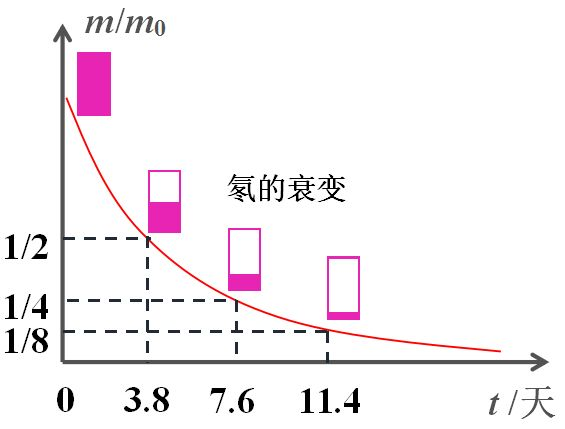
\includegraphics[width=\textwidth,keepaspectratio]{./pictures/20.png}
          \end{minipage}
          \hfill
          \begin{minipage}{0.5\textwidth}
              \begin{enumerate}[label = (\arabic*)]
                  \vspace*{-1em}
                  \item 不同放射性元素的半衰期不同
                        \vspace*{3em}
                  \item 半衰期的大小仅与原子核内部结构有关
                        \vspace*{3em}
                  \item 是对同一元素的大量原子核的统计规律
              \end{enumerate}
          \end{minipage}

          \vspace*{2em}

    \item 人工核反应:
          \begin{enumerate}[label = (\arabic*{})]
              \item 卢瑟福$\alpha$粒子轰击氮原子核发现质子
                    $$
                        \nuc{14}{7}{N} + \nuc{4}{2}{He} \xlra \nuc{17}{8}{O} + \nuc{1}{1}{H}
                    $$
              \item 查德威克$\alpha$粒子轰击铍原子核发现中子
                    $$
                        \nuc{9}{4}{Be} + \nuc{4}{2}{He} \xlra \nuc{12}{6}{C} + \nuc{1}{0}{n}
                    $$
              \item 居里夫人$\alpha$粒子轰击铝原子核发现人工放射性同位素
                    $$
                        \nuc{27}{13}{Al} + \nuc{4}{2}{He} \xlra \nuc{30}{15}{P} + \nuc{1}{0}{n}
                    $$
              \item 居里夫人同时发现正电子
                    $$
                        \nuc{30}{15}{P}  \xlra \nuc{30}{15}{Si} + \nuc{0}{1}{e}
                    $$
          \end{enumerate}

          \vspace*{2em}

    \item 核裂变(链式反应)

          \begin{minipage}{0.26\textwidth}
              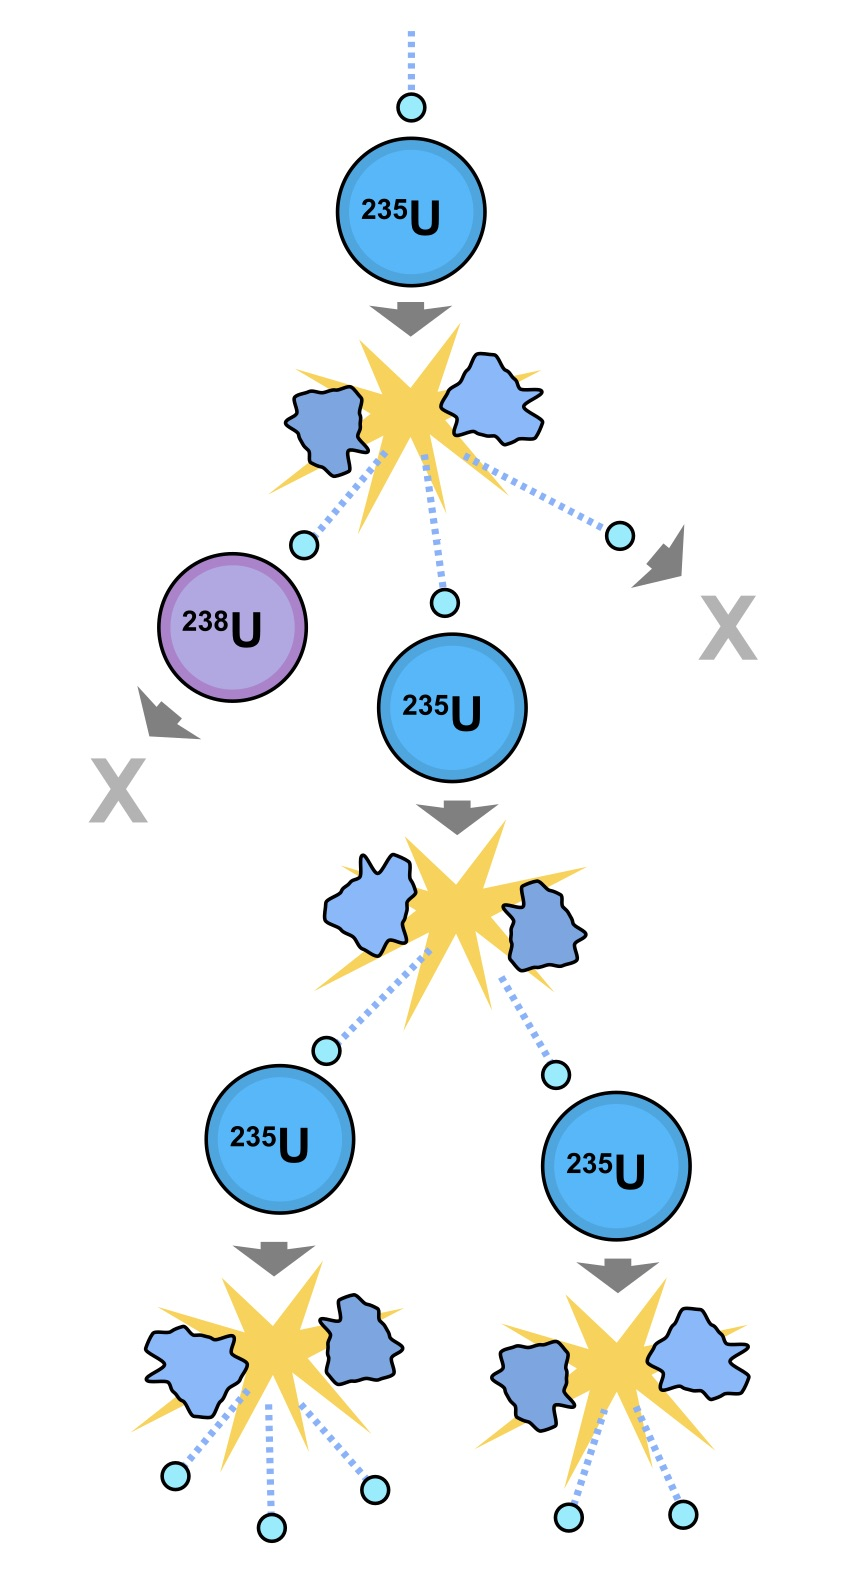
\includegraphics[width=\textwidth,keepaspectratio]{./pictures/21.png}
          \end{minipage}
          \begin{minipage}{0.65\textwidth}
              \begin{enumerate}[label = (\arabic*)]
                  \item $\nuc{235}{92}{U} + \nuc{1}{0}{n} \xlra \nuc{141}{56}{Ba} + \nuc{92}{36}{Kr} + 3\nuc{1}{0}{n}$
                        \vspace*{3em}
                  \item 利用重核裂变的链式反应创造原子弹与可控核电站
                        \vspace*{3em}
                  \item 慢化剂以控制快中子

                        常见慢化剂有石墨,重水,普通水(轻水)
                        \vspace*{3em}
                  \item 氢的同位素: 氕(轻水)$\nuc{1}{1}{H}$,氘(重水)$\nuc{2}{1}{氘}$,氚(超重水)$\nuc{3}{1}{H}$
              \end{enumerate}
          \end{minipage}

          \vspace*{2em}

    \item 核聚变反应(热核反应)

          \begin{itemize}
              \item 将轻核加热使其获得动能以融合,释放出大量能量,以支持其他轻核聚变反应
              \item 氢弹是裂变与聚变反应的结合,通过裂变反应释放的初始热量触发聚变反应
              \item 太阳无时无刻不在发生\textbf{可控核聚变}反应
              \item 核聚变反应的发生过程又可被称为\textbf{热核反应}
          \end{itemize}

          $$
              \nuc{2}{1}{H} + \nuc{3}{1}{H} \xlra \nuc{4}{2}{He} + \nuc{1}{0}{n}
          $$

          \begin{center}
              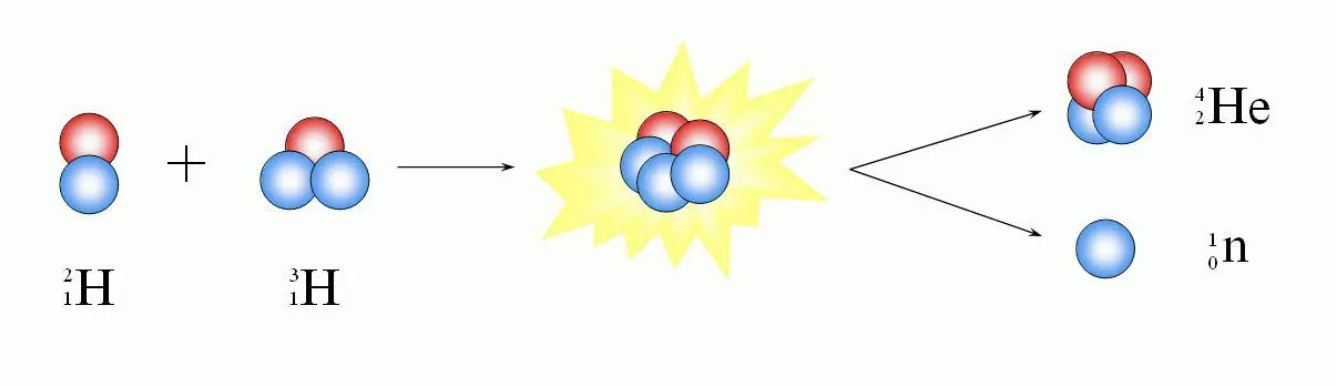
\includegraphics[width=0.7\textwidth]{./pictures/22.png}
          \end{center}
\end{enumerate}

\vspace*{2em}

\subsection{质能方程}
\begin{itemize}
    \item 在核反应方程中\textbf{质量数与质子数是守恒的},但是并\textbf{不代表质量守恒}
    \item 注意平均值的计算并非简单的加和
    \item 质子和中子的质量数均为$1$,但实际质量略有差异
    \item 质能方程: $ E = mc^{2} \quad (m:kg \, E:J)$
    \item 质量单位: $1u$ (原子质量单位,定义为碳原子质量的1/12)
    \item 能量单位: $1MeV$ (兆电子伏特) \quad $1u$相当于$ 931.5 MeV \quad $ $ 1MeV $ 相当于 $10^{6} \cross 1.6 \cross 10^{-19} J  $
\end{itemize}

\subsection{结合能与比结合能}
\begin{enumerate}
    \item 原子核的核子间有一种强大的相互作用力: \textbf{核力}
          \begin{enumerate}[label = (\alph*{})]
              \item 在原子核的尺度内,核力比库伦力要大的多
              \item 核力是短程力,作用范围在$1.5\cross10^{-15}$之内

                    (大于此距离表现为吸引力,小于此距离表现为排斥力,因此不会完全融合)

                    \vspace{-1em}
                    \begin{adjustbox}{minipage=0.92\linewidth, bgcolor=gray!20, padding=1em}
                        \small % 将字号变小为 small
                        自然界中较轻原子核,质子数与中子数大致相等,对于较重原子核,中子数大于质子数,越
                        重元素相差越多
                    \end{adjustbox}
                    \vspace{-1em}

          \end{enumerate}

    \item 结合能: 原子核是核子结合构成的,要把它们分开所需要的能量称之为原子核的结合能

          原子核越大,它的结合能就越大,所以有意义的应该是结合能与核子数的比值

    \item 比结合能: 比结合能越大,表示核子结合越牢,原子核越稳定(具备更低的能量状态)

\end{enumerate}


\end{document}